\cleardoublepage

\chapter{Testing in Quantum}
\label{Ch3:QTesting}

After providing a brief introduction to quantum computing, let us allocate some time to delve into the latest developments in the field of quantum testing. This section will be divided into two different perspectives. Firstly, we will explore the testing of Quantum Platforms, with a specific focus on Qiskit and how it can evolve for different platforms. Subsequently, we will continue with various approaches and techniques for testing quantum programs, hereafter referred to as QP.

\section{Quantum computing platforms}
\label{Ch3.1:TQPlat}

As mentioned earlier, we will begin by examining the testing of quantum platforms. We will introduce these approaches in chronological order and the authors will even assess how they compare to each other, observing improvements over time.

\subsection{QDiff; 15-19 November 2021}
\label{Ch3.1.1:QDiff}

QDiff, differential testing of quantum software stacks (QSS), is the approached presented by Jiyuan Wang et all. in their 2021 article titled \textit{"QDiff: differential testing of quantum software stacks"}\cite{wang2021qdiff}, they introduce it as a novel differential testing technique for QSS.\newline

Their motivation behind this work arises from the increasing interest in quantum computing and the development of QSS as a high-level languages for quantum programming. These languages aim to shield users from the mathematical and physical complexities inherent in quantum computing. Another motivation is to offer a potential solution for identifying failures within QSS, which aids in resolving the confusion and incoherence that often arises when a user reports bugs. When reviewing the collection of issues reported for each QSS, these problems frequently reveal inconsistencies in identifying the potential source of the bug or determining whether the issue originates from the probabilistic or noisy nature of quantum indeterminacy. \newline

The authors idea is to be able to perform testing in the three most widely used QSS \cite{larose2019overview} at that time: Qiskit, Cirq and Pyquil. Now, let us explore the workflow (Figure \ref{Fig:QDiffWorkOverflow}) and key innovations in  QDiff, which will include their propose solutions for technical challenges that complicate testing within QSS.

\begin{itemize}
    \item QP generator: In order to fulfil our needs while testing QSS, we need to generate semantically equivalent programs. The authors proposed a set of equivalent gate transformation rules designed to preserve program semantics. These seven rules have been derived from a detail analysis of each gate and their behaviour when deployed sequentially.
    \begin{figure}[H]
        \centering
        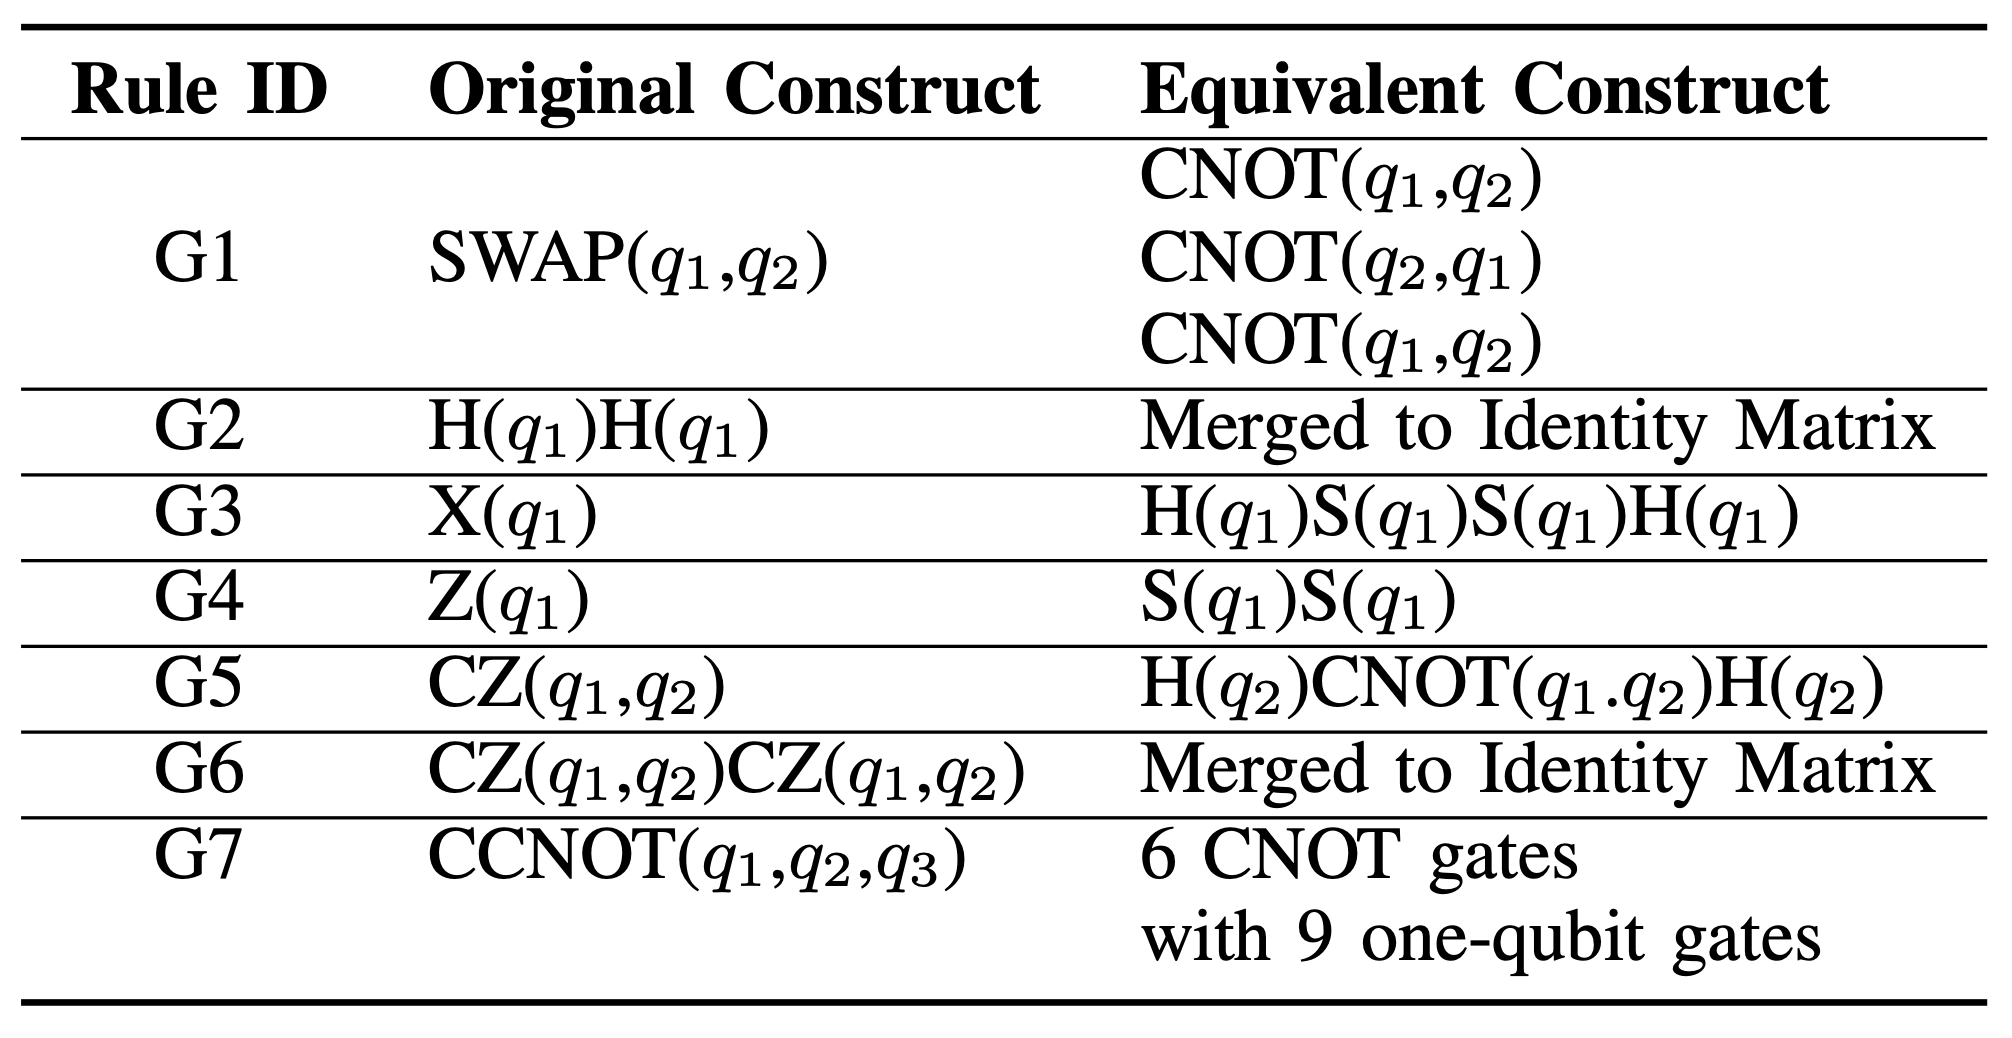
\includegraphics[width=0.6\textwidth]{TFM/photos/QDiffRules.png}
        \caption{Semantic preserving rules \cite{wang2021qdiff}} 
        \label{Fig:QDiffRules}
    \end{figure}

    Followed by mutation modifications, QDiff utilises this process to diversify the pool of input programs. The initial seed consists of 6 QPs, and through mutation, it will be expanded to 730 variants. Quantum mutant operators used in QDiff:
        \begin{itemize}
            \item[] M1: Gate insertion/deletion.
            \item[] M2: Gate change.
            \item[] M3: Gate swap.
            \item[] M4: Qubit change.
        \end{itemize}

    \item Filtering QP based on whether they are worth running. This determination relies on the execution system and the specific QP. A circuit is deemed suitable for execution on quantum hardware or a noisy simulator if it adheres to two key thresholds:
    
    \begin{itemize}
        \item[-] The maximum number of gates, determined by average execution gate and T1 time for the system, where T1 represents the decoherence time for a qubit. 
        \item[-] The maximum number of 2-qubit gates, determined by the error rate tolerance willing to be added by the user  the final measurements 
    \end{itemize}

    A concrete example of these boundaries is provided in \textit{IV. QDIFF APPROACH - B. Quantum Simulation and Hardware Execution} \cite{wang2021qdiff}.

    \item Comparing outcomes derived from two equivalent quantum programs. The authors employ two similar techniques discussed in \textit{IV. QDIFF APPROACH - C. Equivalence Checking via Distribution Comparison} \cite{wang2021qdiff} and prior works \cite{chan2014optimal}\cite{aaronson2016complexity}\cite{cross2019validating}. Let use outline both methods.\newline
    
    Firstly, it is imperative to establish a threshold $t$ representing the maximum acceptable distance and a significance level $p$. Afterwards, the minimum number of executions required for statistically guaranteed comparison is calculated. Following the executions, empirical distribution functions (EDFs) are computed.

    \begin{itemize}
        \item[-] Kolmogorov-Smirnov (K-S) distance: This metric characterise the K-S distance as the most substantial difference between the two EDFs. If this difference is less than $t$, the QPs are deemed similar.
        \item[-] Cross entropy: The comparison involves evaluating the total entropy of both EDFs, equally constrained by the threshold $t$.
    \end{itemize}

    \item Reporting divergences. Once a divergence has been found, the system will identify the difference between both QPs. Then it difference between: backend, frontend and API gate implementation.
    
    \begin{figure}[H]
        \centering
        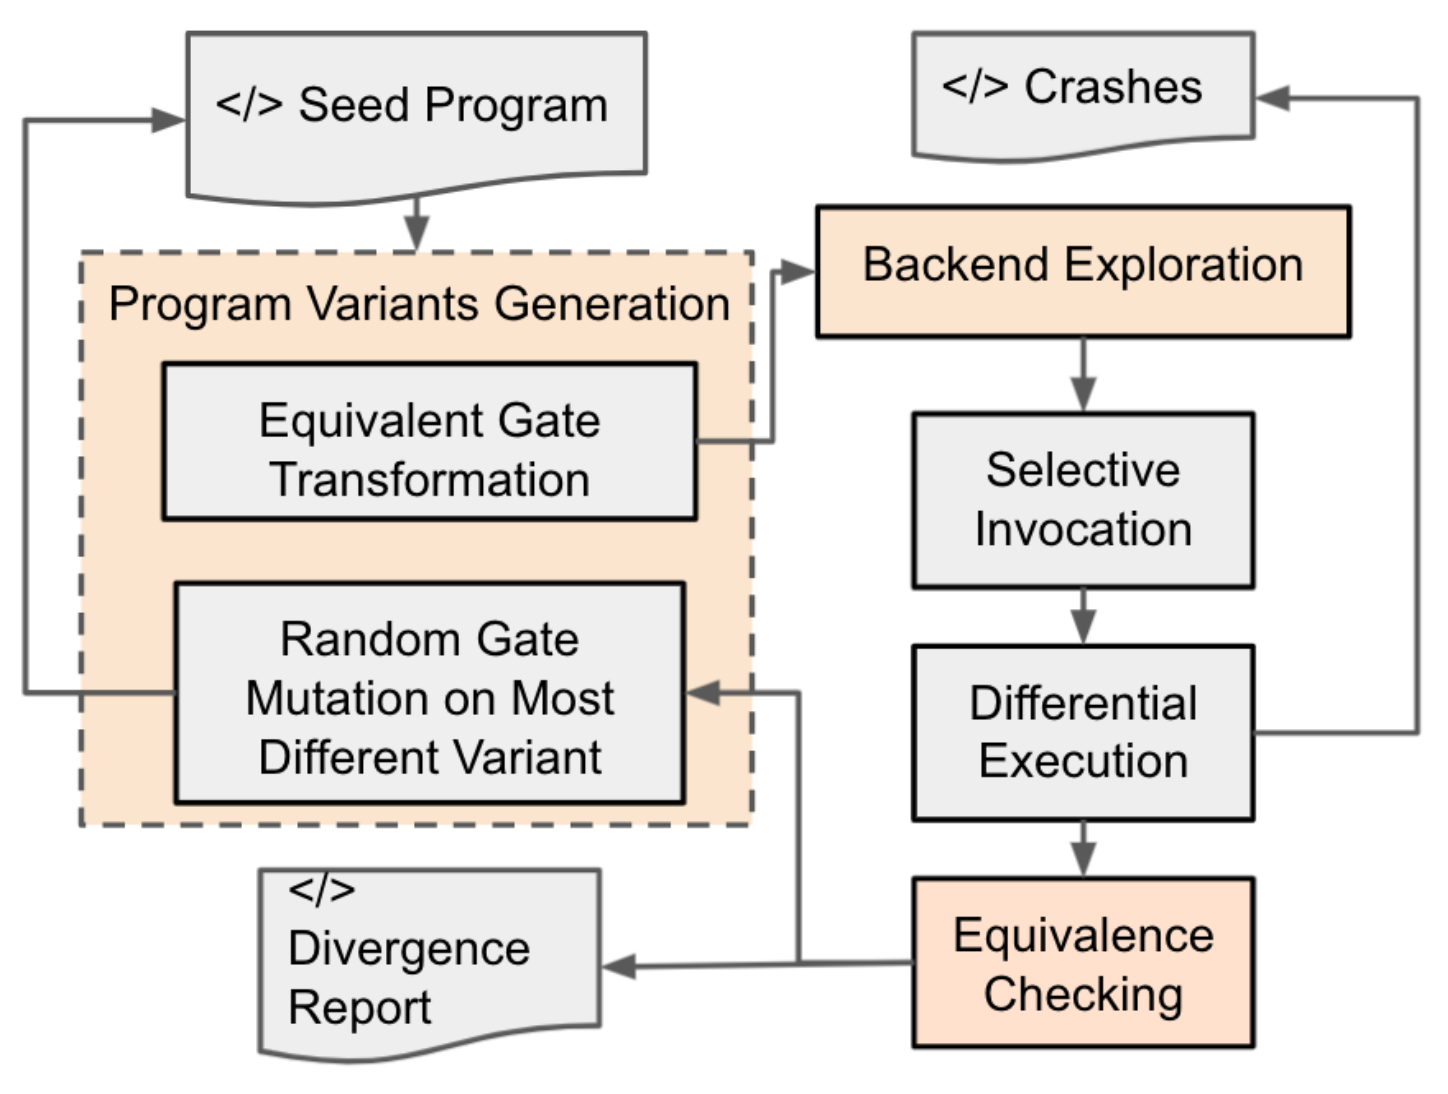
\includegraphics[width=0.6\textwidth]{TFM/photos/QDiffWorkoverflow.png}
        \caption{QDiff overview \cite{wang2021qdiff}} 
        \label{Fig:QDiffWorkOverflow}
    \end{figure}

    We should now conclude by highlighting the key contributions and outcomes of these experiments:

\begin{itemize}
    \item QDiff successfully evaluated more than one QSS.
    \item A total of 14799 QPs were generated, organised into 730 sets of semantically equivalent circuits.
    \item Among the 730 sets, 33 differing outcomes were identified, all which will undergo manual checking.
    \begin{itemize}
        \item[-] Out of these, 4 discrepancies resulted in simulator crashes, while the remaining divergences exceeded expected noise levels on IBM hardware.
        \item[-] Six distinct sources of instability were identified, comprising 4 software crash bugs in Pyquil and Cirq, along with 2 root causes potentially explaining 25 out of 29 cases of divergence beyond anticipated noise on IBM hardware, attributed to unreliable connections between two qubits.
    \end{itemize}
    
\end{itemize}

\vspace{15pt}
\subsection{Sequence to Sequence model for QSharp ; 04-13 April 2022}

Trinca et al. presented the paper with title \textit{"A Preliminary Study on Generating Well-Formed
$Q\#$ Quantum Programs for Fuzz Testing"} \cite{trinca2022preliminary}

\vspace{15pt}
\subsection{Multi-lingual property based approach; May 2022}

A multi-lingual benchmark for property-based testing of quantum programs \cite{pontolillo2022multi}

\vspace{15pt}
\subsection{QSS review; May 2022}
Matteo Paltenghi presented his paper titled \textit{"Cross-Platform Testing of Quantum Computing Platforms"} in 2022, as documented in \cite{paltenghi2022cross}. The primary objective of this paper is to delineate the challenges faced by quantum computing platform testing in 2022, offering hypotheses on potential solutions. We could consider this paper as the seed for Paltenghi's subsequent research with MorphQ, the finding of which will be presented upon shortly. Let us explore the challenges and hypotheses outlined by the author.

\vspace{-10pt}
\begin{itemize}
    \item[] \textbf{Challenge} 1: Quantum program generation. Platform testing requires a large amount of programs. However, there is only a few real quantum program examples available nowadays \cite{campos2021qbugs}.
    \item[] \textbf{Challenge} 2: Multi-platform Program Translator. Quantum programs are often written in new programming languages or expressed using APIs on top of existing languages. The absence of standardized intermediate representations presents a challenge for cross-platform testing. Attempts have been made with \textit{OpenQASM} \cite{cross2017open}\cite{cross2022openqasm}.
    \item[] \textbf{Challenge} 3: Multivariate Binary Distribution Comparison. The probabilistic nature of quantum measurements introduces complexity to testing, as outputs are represented by distributions. Research has been conducted on this challenge in quantum debugging \cite{huang2018qdb}\cite{huang2019statistical}\cite{li2020projection} , along with preliminary work using Kolmogorov-Smirnov or cross-entropy tests \cite{wang2021qdiff}.
\end{itemize}

\vspace{-10pt}
\begin{itemize}
    \item[] \textbf{Hypothesis} 1: Cross-platform testing can be a promising direction to find bugs in QC platforms. The authors suggest the existence of bugs in traditional buggy components, such as compilers and optimizers, building on the work presented by Wang et al. \cite{wang2021qdiff}.
    \item[] \textbf{Hypothesis} 2: Testing with automatically generated realistic quantum programs could boost the effectiveness of current differential testing on QC platforms.
    \item[] \textbf{Hypothesis} 3: Machine learning methods could be successful in generating realistic quantum programs. This hypothesis comes from classical computing and how genetic algorithms have been used for program synthesis \cite{koza1994genetic} and reinforcement learning to generate equivalent quantum programs \cite{moro2021quantum}.
    \item[] \textbf{Hypothesis} 4: The quantum programs can be translated to run on multiple platforms.
    \item[] \textbf{Hypothesis} 5: A statistical test specific for multivariate binary distribution should perform better than existing unspecialised methods.
\end{itemize}

After outlining these brief ideas about the challenges and potential solutions in quantum platform testing, let's proceed to introduce the subsequent work by the same author.

\subsection{MorphQ; 14-20 May 2023}
\label{Ch3.1.2:MorphQ}
Matteo Paltenghi and Michael Pradel presented in May 2023 their latest work on testing QQS, introducing metamorphic testing as a novel approach for quantum platforms. Their innovative method involves the design of metamorphic rules for Qiskit.3 Their article, titled: \textit{"MorphQ: Metamorphic testing of the qiskit quantum computing platform"} \cite{paltenghi2023morphq}, further develops this concept, presenting a fresh perspective on generating quantum programs using a defined grammar. This advancement brings us closer to the idea of automating the testing process, eliminating the need for a library of quantum programs as generation seed, which was the traditional approach up to this point.\newline

MorphQ will focus on Qiskit, as quantum platform, employing metamorphic testing to address specific challenges presented in quantum computing. The oracle problem will be avoided as it will be resolved by the use of MR, eliminating the need for a detailed specification of expected input behaviour. Let us provide a general overview of MorphQ as presented by the authors, then we will focus on the key innovations within each of its distinct components .

\begin{figure}[H]
        \centering
        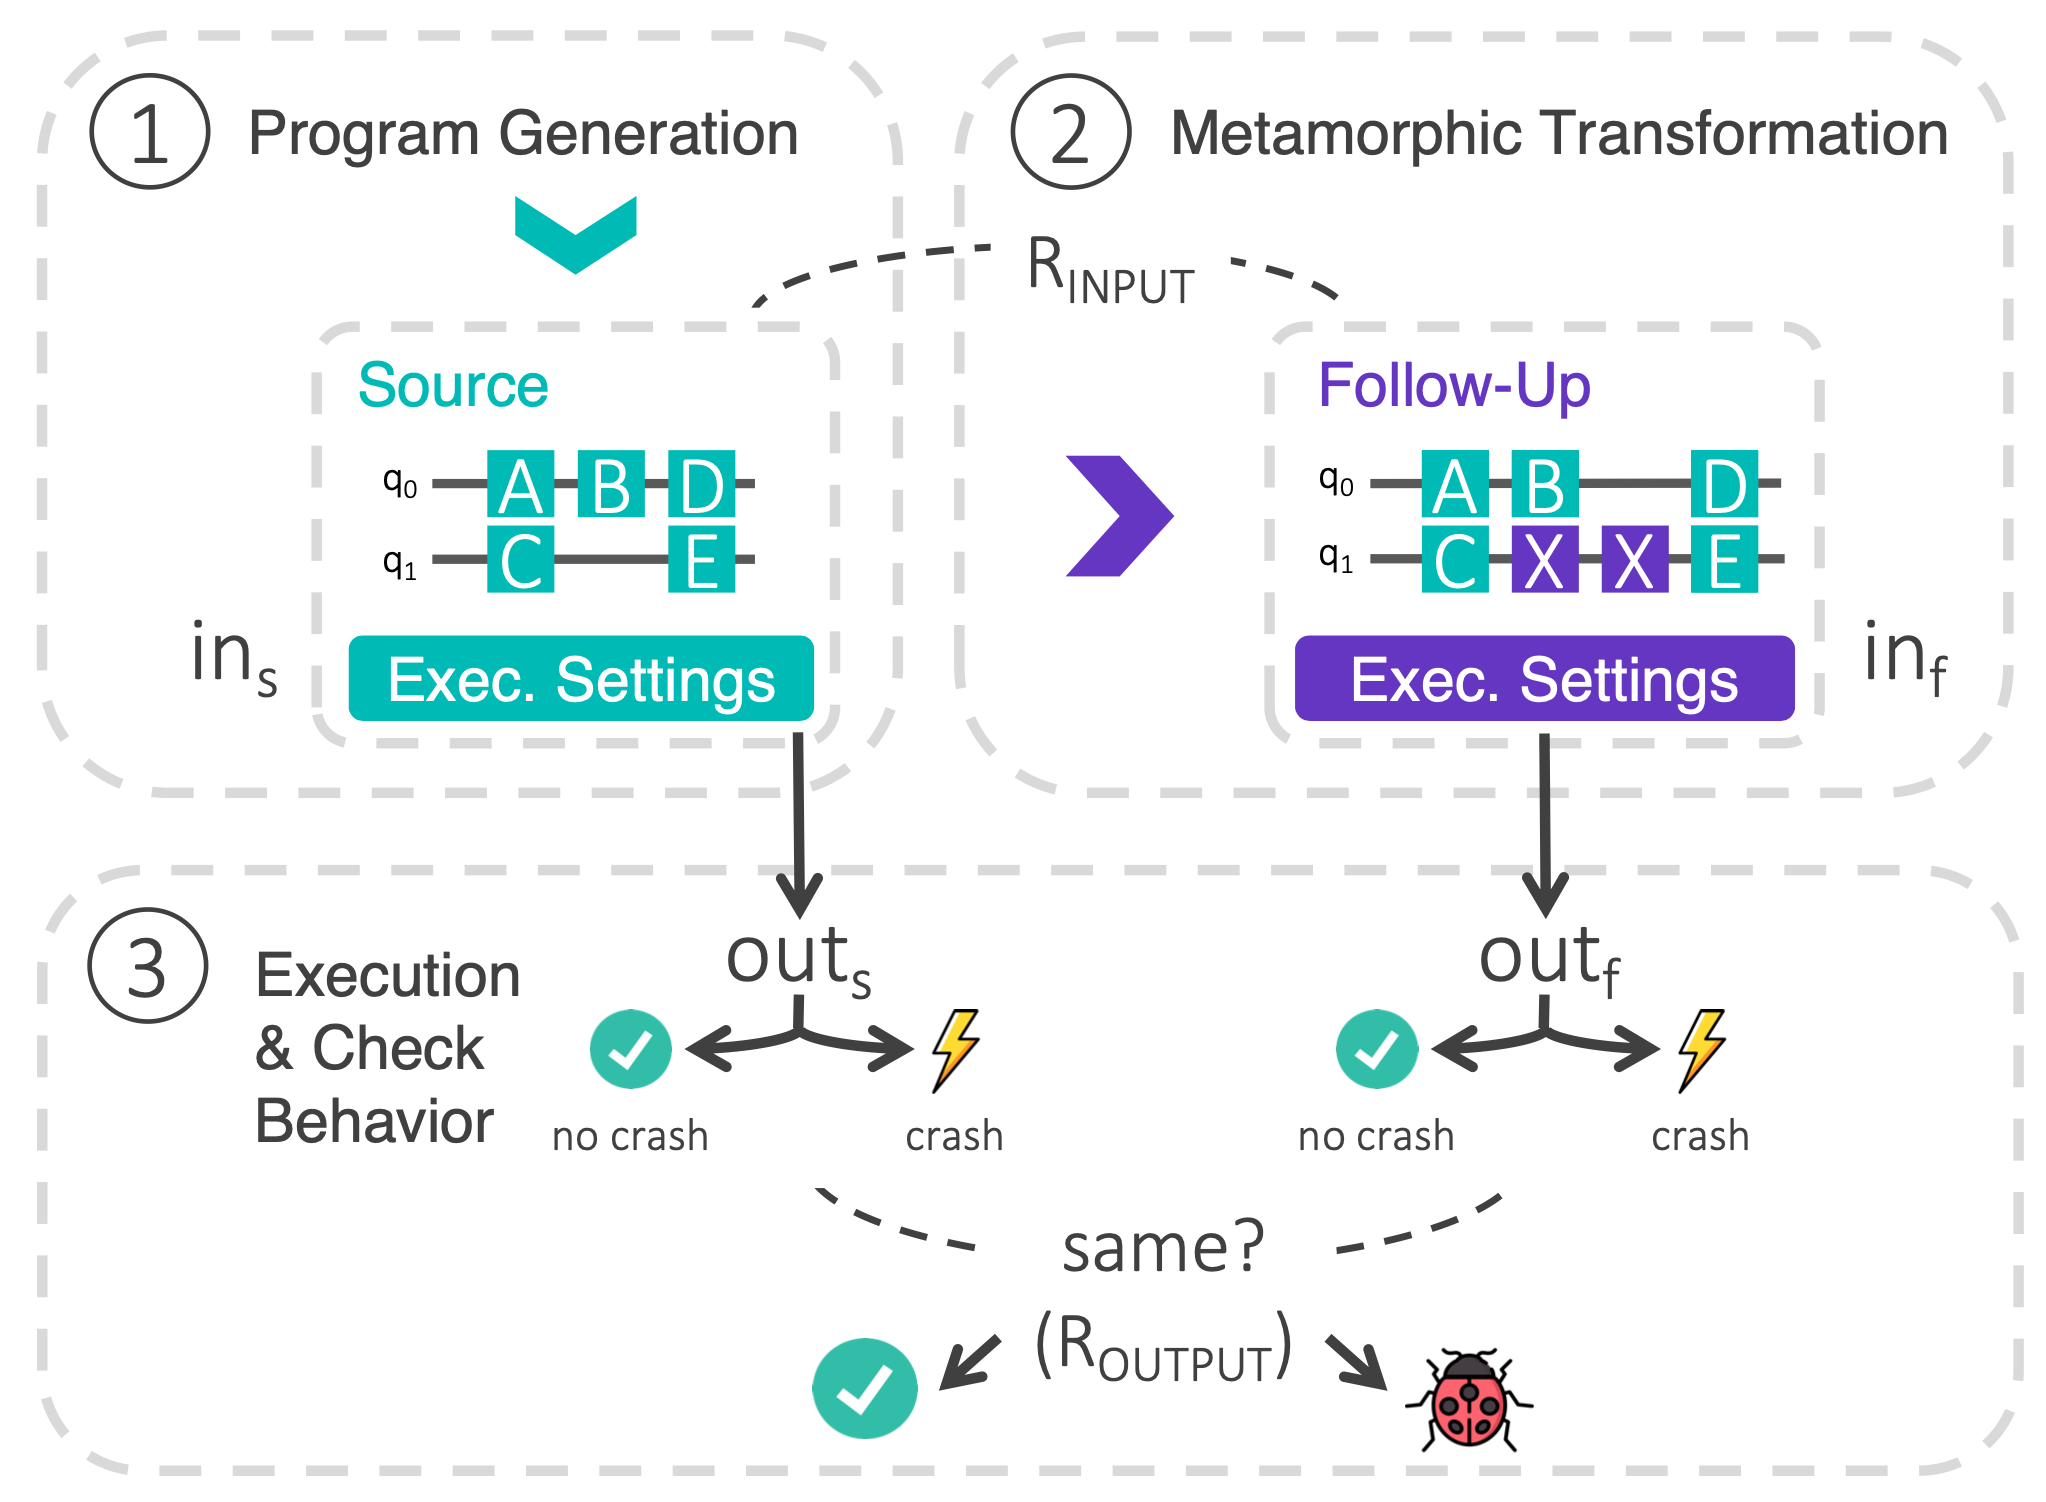
\includegraphics[width=0.58\textwidth]{TFM/photos/MorphQOverview.png}
        \caption{MorphQ overview \cite{paltenghi2023morphq}} 
        \label{Fig:MorphQOverview}
\end{figure}

\vspace{-12pt}
As previously mentioned, one of the authors' significant contributions lies in their approach to program generation. Since the focus is on testing the quantum platform, the primary objective of this proposal is to create syntactically correct quantum programs, thus preventing execution crashes. These this automating generated programs will serve as test suit for the QSS. To begin, Paltenghi and Pradel introduced the grammar that will guide the program generation process. This grammar follows the typical recursive structure found in computing. A subset of it is illustrated in Figure \ref{Fig:MorphQGrammar}, as provided by the authors in their paper. You can access all the related information about the grammar and the rest of the article on their \hyperlink{https://github.com/sola-st/MorphQ-Quantum-Qiskit-Testing-ICSE-23}{GitHub} page. (Visible link, hided link, footnote, both?)

\vspace{-8pt}
\begin{figure}[H]
        \centering
        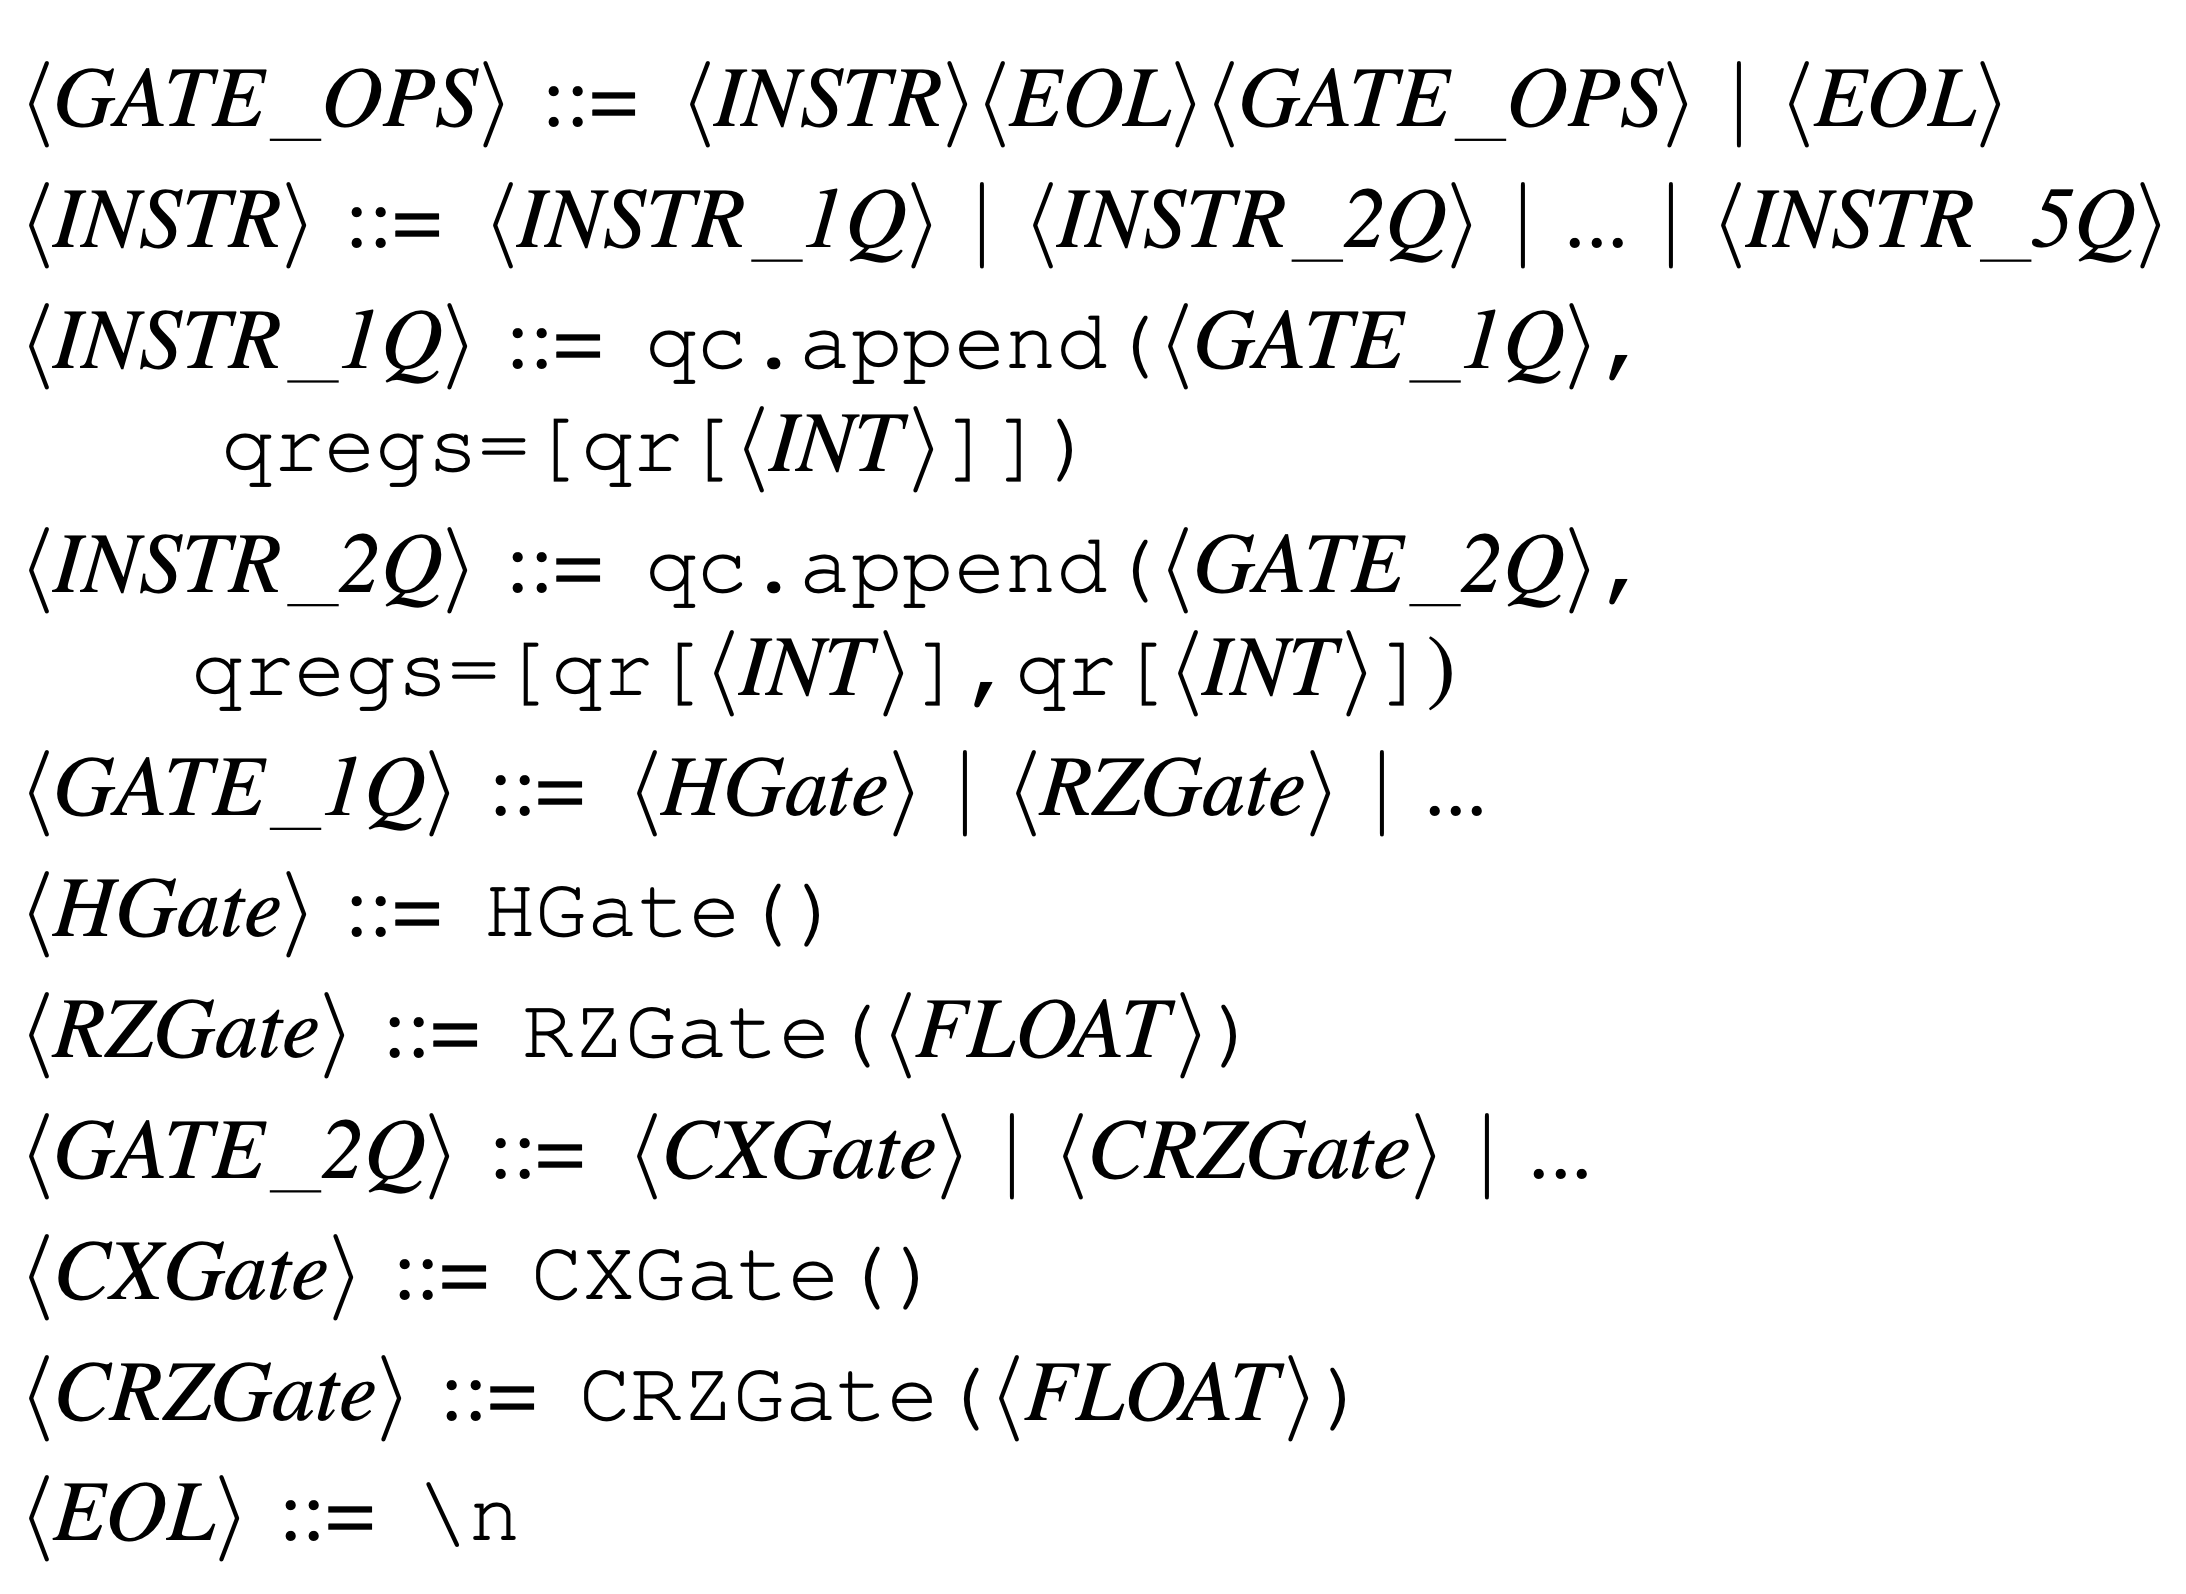
\includegraphics[width=0.56\textwidth]{TFM/photos/MorphQGrammar.png}
        \caption{Subset of the QP generation grammar \cite{paltenghi2023morphq}} 
        \label{Fig:MorphQGrammar}
\end{figure}

The purpose of defining this grammar is to ensure that invalid quantum programs are avoided. A random approach would not be ideal, as it would likely generate a high number of invalid programs. Additionally, the authors will impose a constraint on the number of gates per program, limiting it to 30. Higher amount of gates can increase considerably the execution time due to the complexity of quantum operations. Their commitment towards keeping execution times within reasonable limits, lies in the decision of the authors to only use simulators, where the size of the matrix defining a single operator grows exponentially with the number of qubits involved.\newline

Once we have been able to generate the source input for the testing desired, the authors defined the metamorphic rules that Qiskit should fulfil classifying them in 3 categories: Circuit transformation which modify the circuit, representation transformations which change the intermediate representation of QP and execution transformations, which affect the execution environment, we could observe this metamorphic rules in Figure \ref{Fig:MorphQMR}. 

\begin{figure}[H]
        \centering
        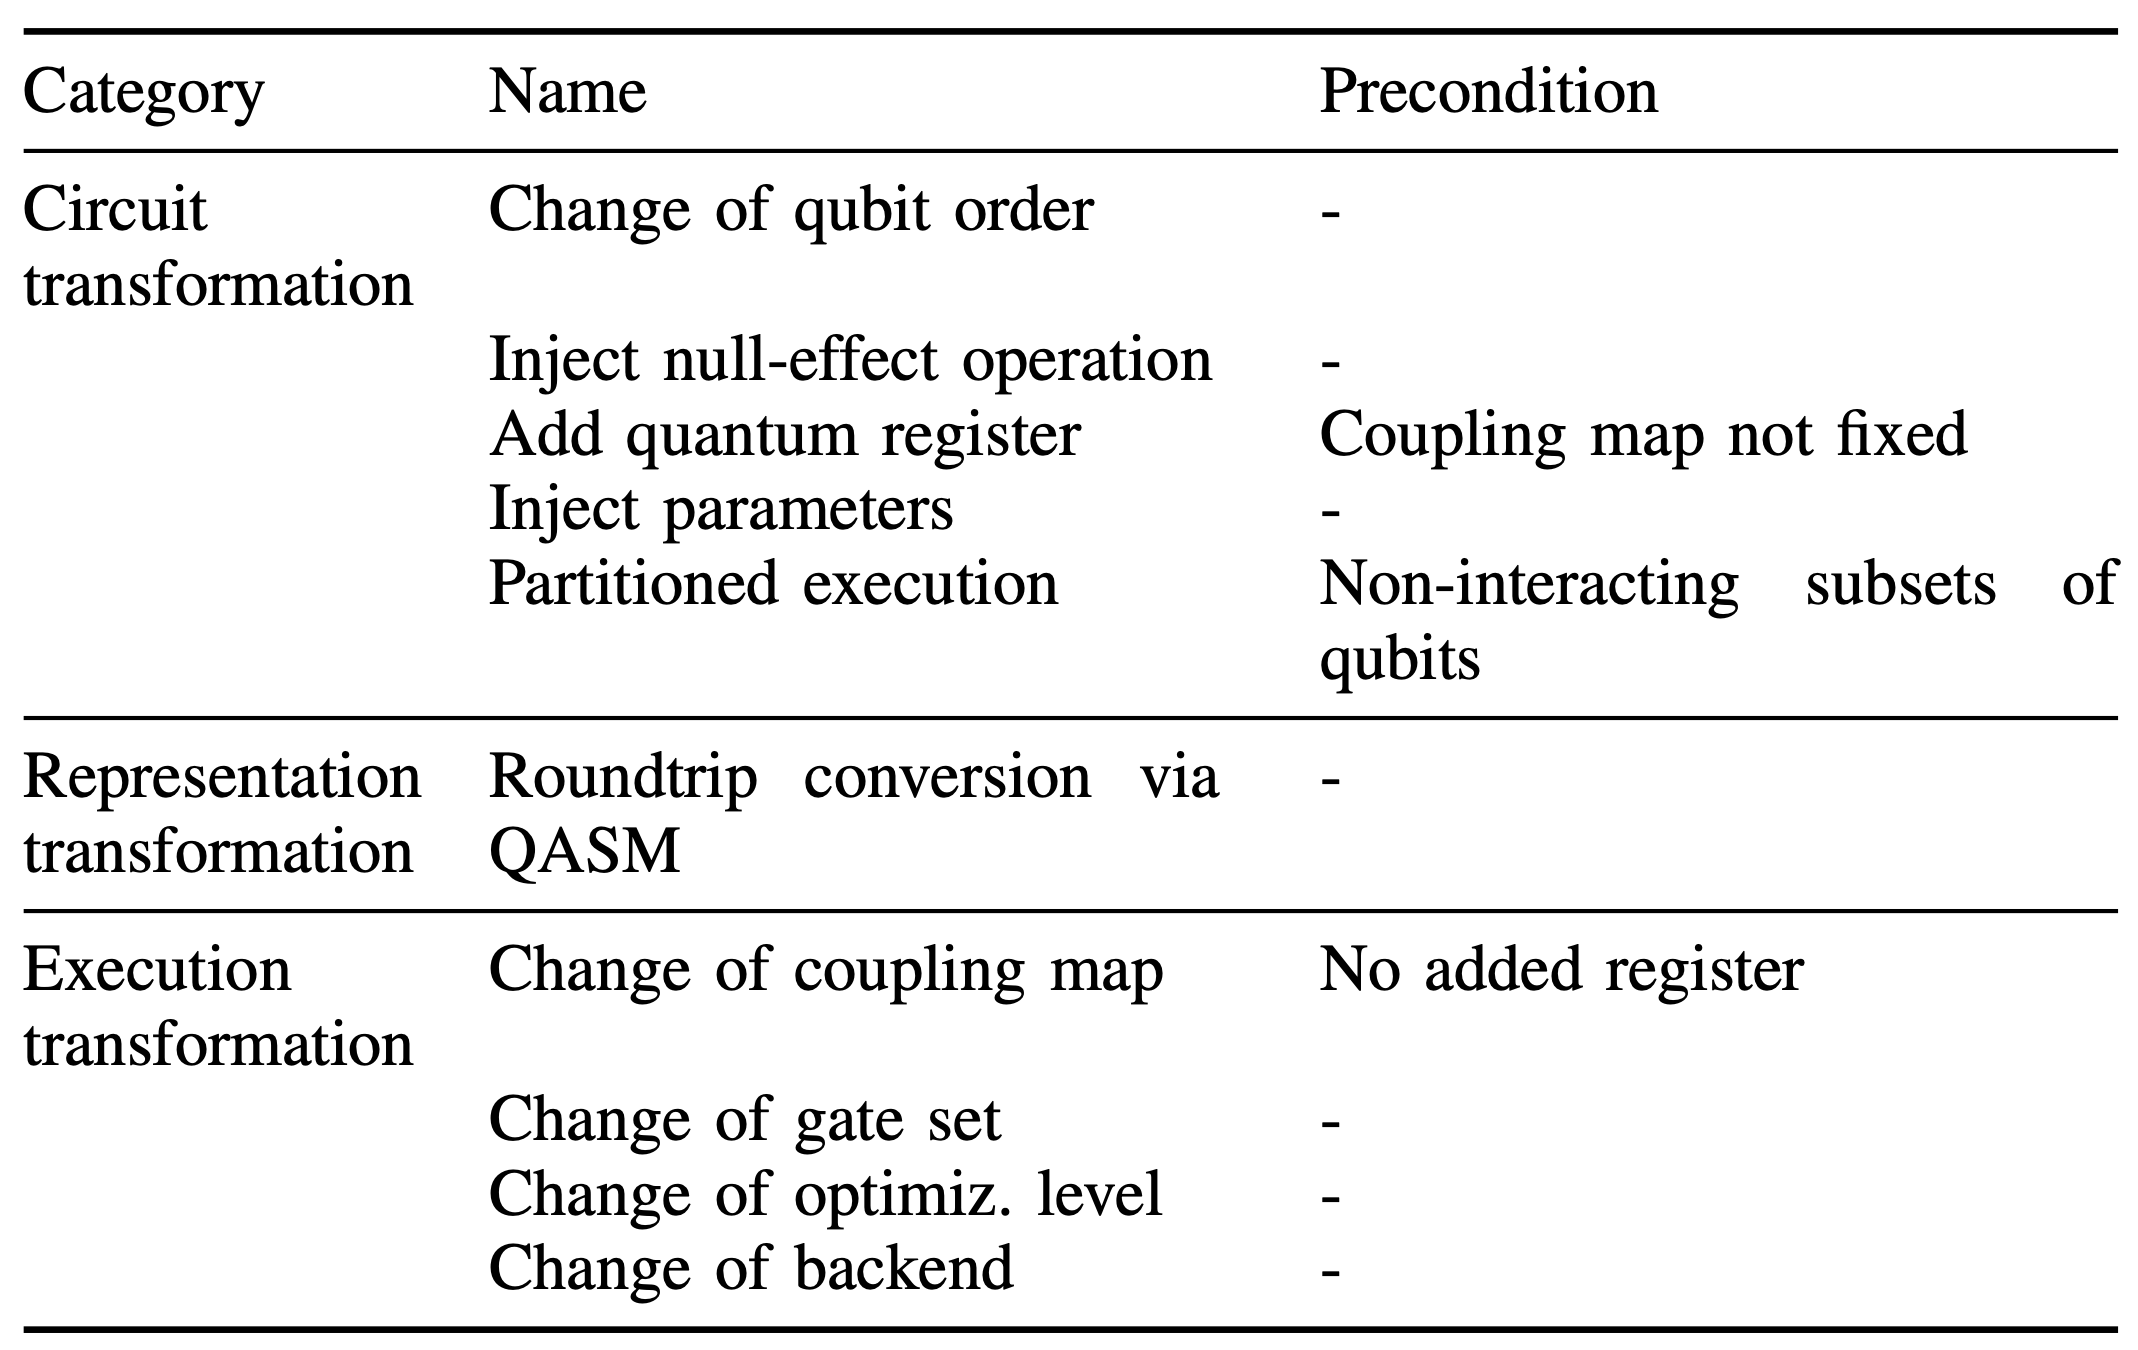
\includegraphics[width=0.6\textwidth]{TFM/photos/MorphQMR.png}
        \caption{Qiskit MR used by QMorph \cite{paltenghi2023morphq}} 
        \label{Fig:MorphQMR}
\end{figure}

The expected relationship between source and follow-up outputs is "equivalence", with the only exception of non-semantic-preserving transformations, specifically, the change of qubit order and partitioned execution which will need a posterior treatment before comparing behaviours. This is why we will continue applying metamorphic transformations unless one of the exceptions mentioned above is introduced. This transformations are executed through python AST or/and sectioning source code with python matching technique, adding needed elements and reconstructing the code.\newline

In the final step of MorphQ, which involves execution and behaviour checks, the primary assessment is crash check. Identifying a crash in the follow-up program marks a critical failure. As we are all aware, when executing quantum programs without accounting for quantum noises, the result can be non-deterministic linked to the final state amplitudes, reflecting the well-known probabilistic nature of quantum measurement. Consequently, we would need to execute the programs a specific number of shots to compare two different distributions and decide if the output is "equivalent" or we have possibly found a failure. To determine this 
required number of executions, the authors follow the same technique as the one used in QDiff, employing the \textbf{L1 norm }\cite{chan2014optimal}. The distribution are compared using Kolmogorov-Smirnov test (p-value < 5\%)\newline
 
Another noteworthy aspect is the management of warning messages related to crashes. The authors implemented a semi-automatic clustering approach for these warnings, aiming to abstract from program-specific references. Afterwards, a random selection process is applied to each cluster, and the chosen programs undergo manual inspection. During these inspections, transformations are reversed step by step until the one responsible for the fault is reached. Then, they use \textbf{delta debugging} until they identify the minimal sequence of operations to trigger the crash. \newline

Let us summarise the key results and contributions of MorphQ, keeping in mind that the experiments were constrained by a 48-hour execution time-frame. The authors also adapted QDiff to the same execution time-frame to be able to compare results.

\begin{itemize}
    \item QP generator:
    \begin{itemize}
        \item Automatically generated 8360 quantum programs .
        \item Source-QP executed without crashing.
        \item Wide range of programs produced (Figure \ref{Fig:MorpgQDiverQP}). 
        \item Higher code coverage vs QDiff: 8.1\% vs 6.1\% 
    \end{itemize}
    \item 13 bugs discovered in the latest version of Qiskit.
    \item Follow-up QP behaviour analysis:
    \begin{itemize}
        \item Crashed in 23.2\% of the cases,with only 56 programs showing a distribution difference.
        \item Demonstrated wider diversity compared to QDiff, as measured by unique API calls.
        \item \textit{Roundtrip conversion via QASM} and \textit{Inject null-effect operations} are the most effective MR, althogh a combination of several MR will produce better results, exposing 8 out of 13 bugs (Figure \ref{Fig:MorpgQDiverQP}). 
        \item Non-crashing follow-up QP: Upon evaluating the 56 programs, it was determined that the differences in distribution were due to randomness, which is plausible given the test's significance level.
    \end{itemize}
    \item False positive: MorphQ may generate false positive warnings because the MR do not always hold in practice, even when is theoretically sound. This can occur when applying the \textit{Change of gate set}. In Qiskit, A* algorithm is used to find equivalent gates, although exploring all possibilities is impractical. Therefore, we might encounter the warning \textit{"Unable to map source basis to target basis"}, which  could be recognised as a limitation of the platform.
\end{itemize}

\begin{figure}[!tbp]
  \centering
  \begin{minipage}[b]{0.36\textwidth}
    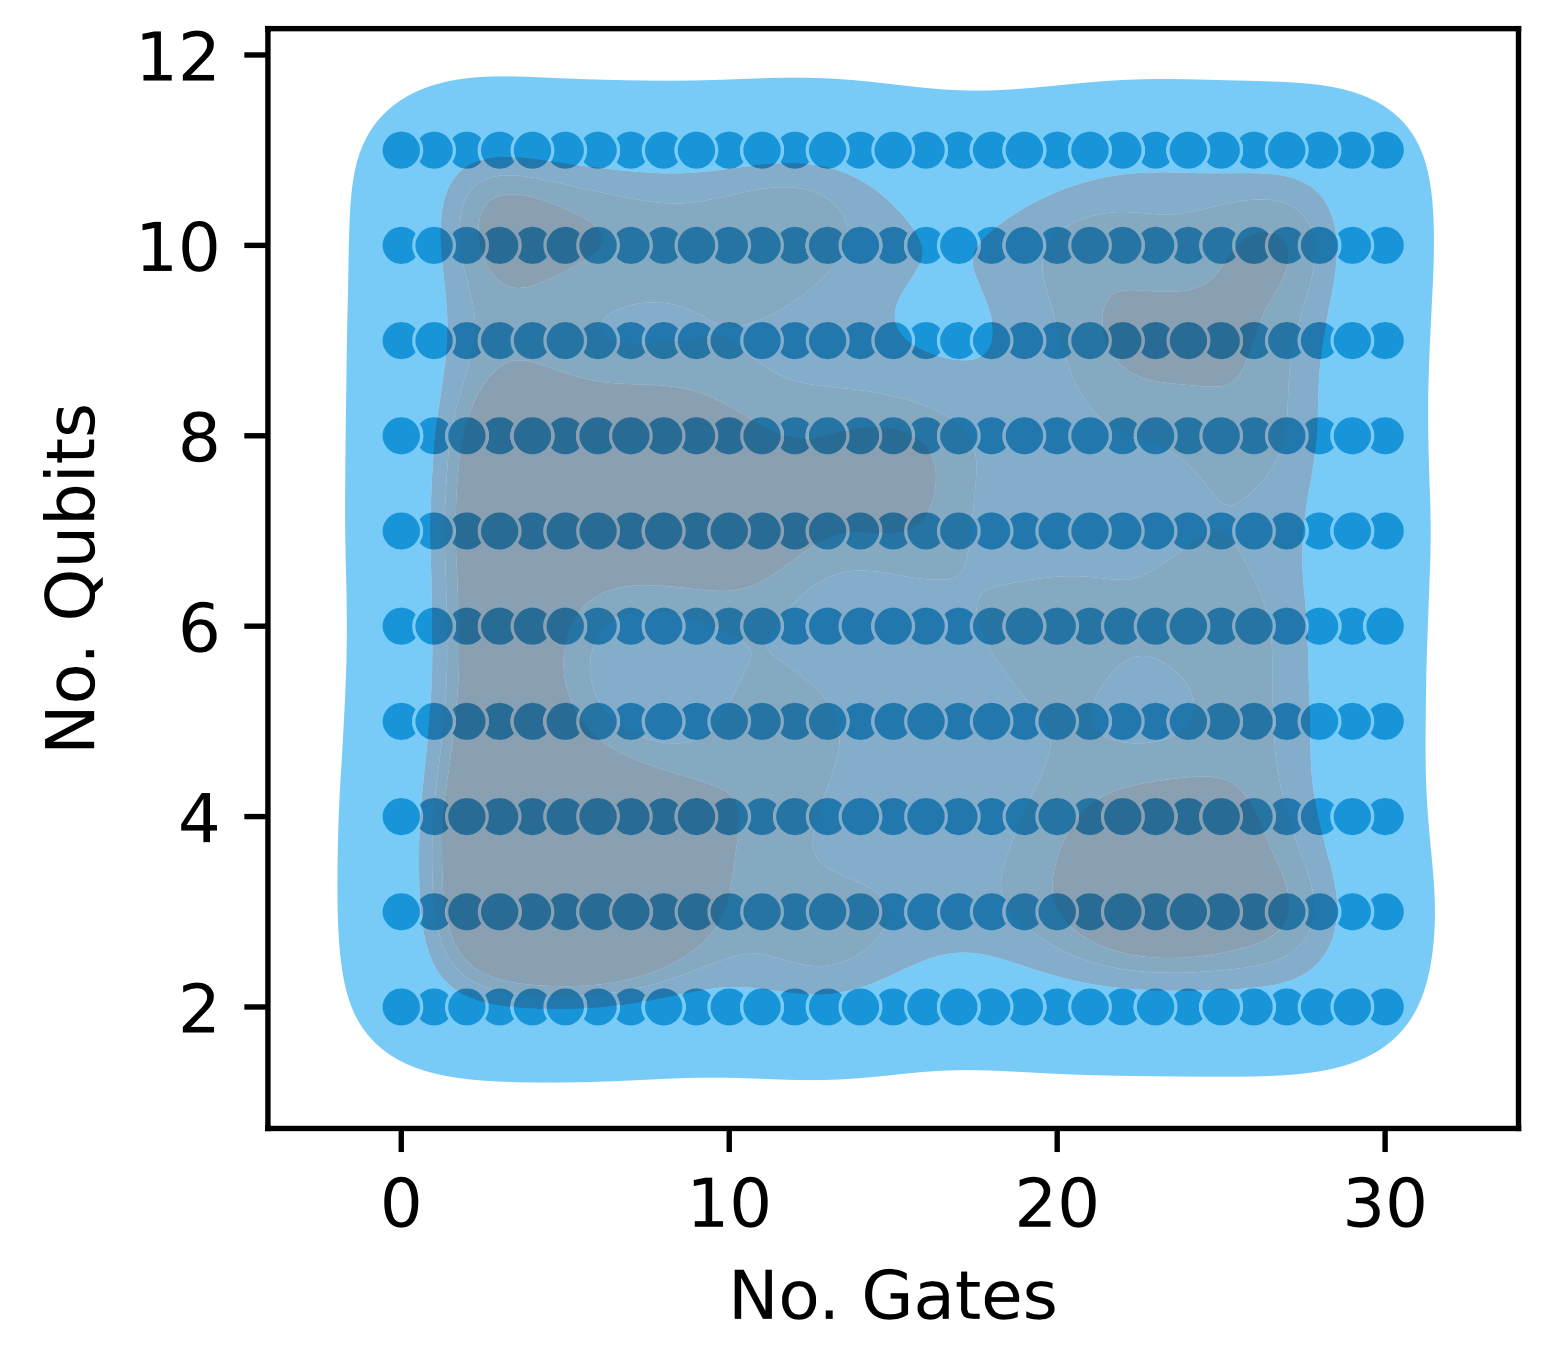
\includegraphics[width=\textwidth]{TFM/photos/MorpgQDiverQP.png}
    \caption{QP diversity \cite{paltenghi2023morphq}.} 
    \label{Fig:MorpgQDiverQP}
  \end{minipage}
  \hfill
  \begin{minipage}[b]{0.55\textwidth}
    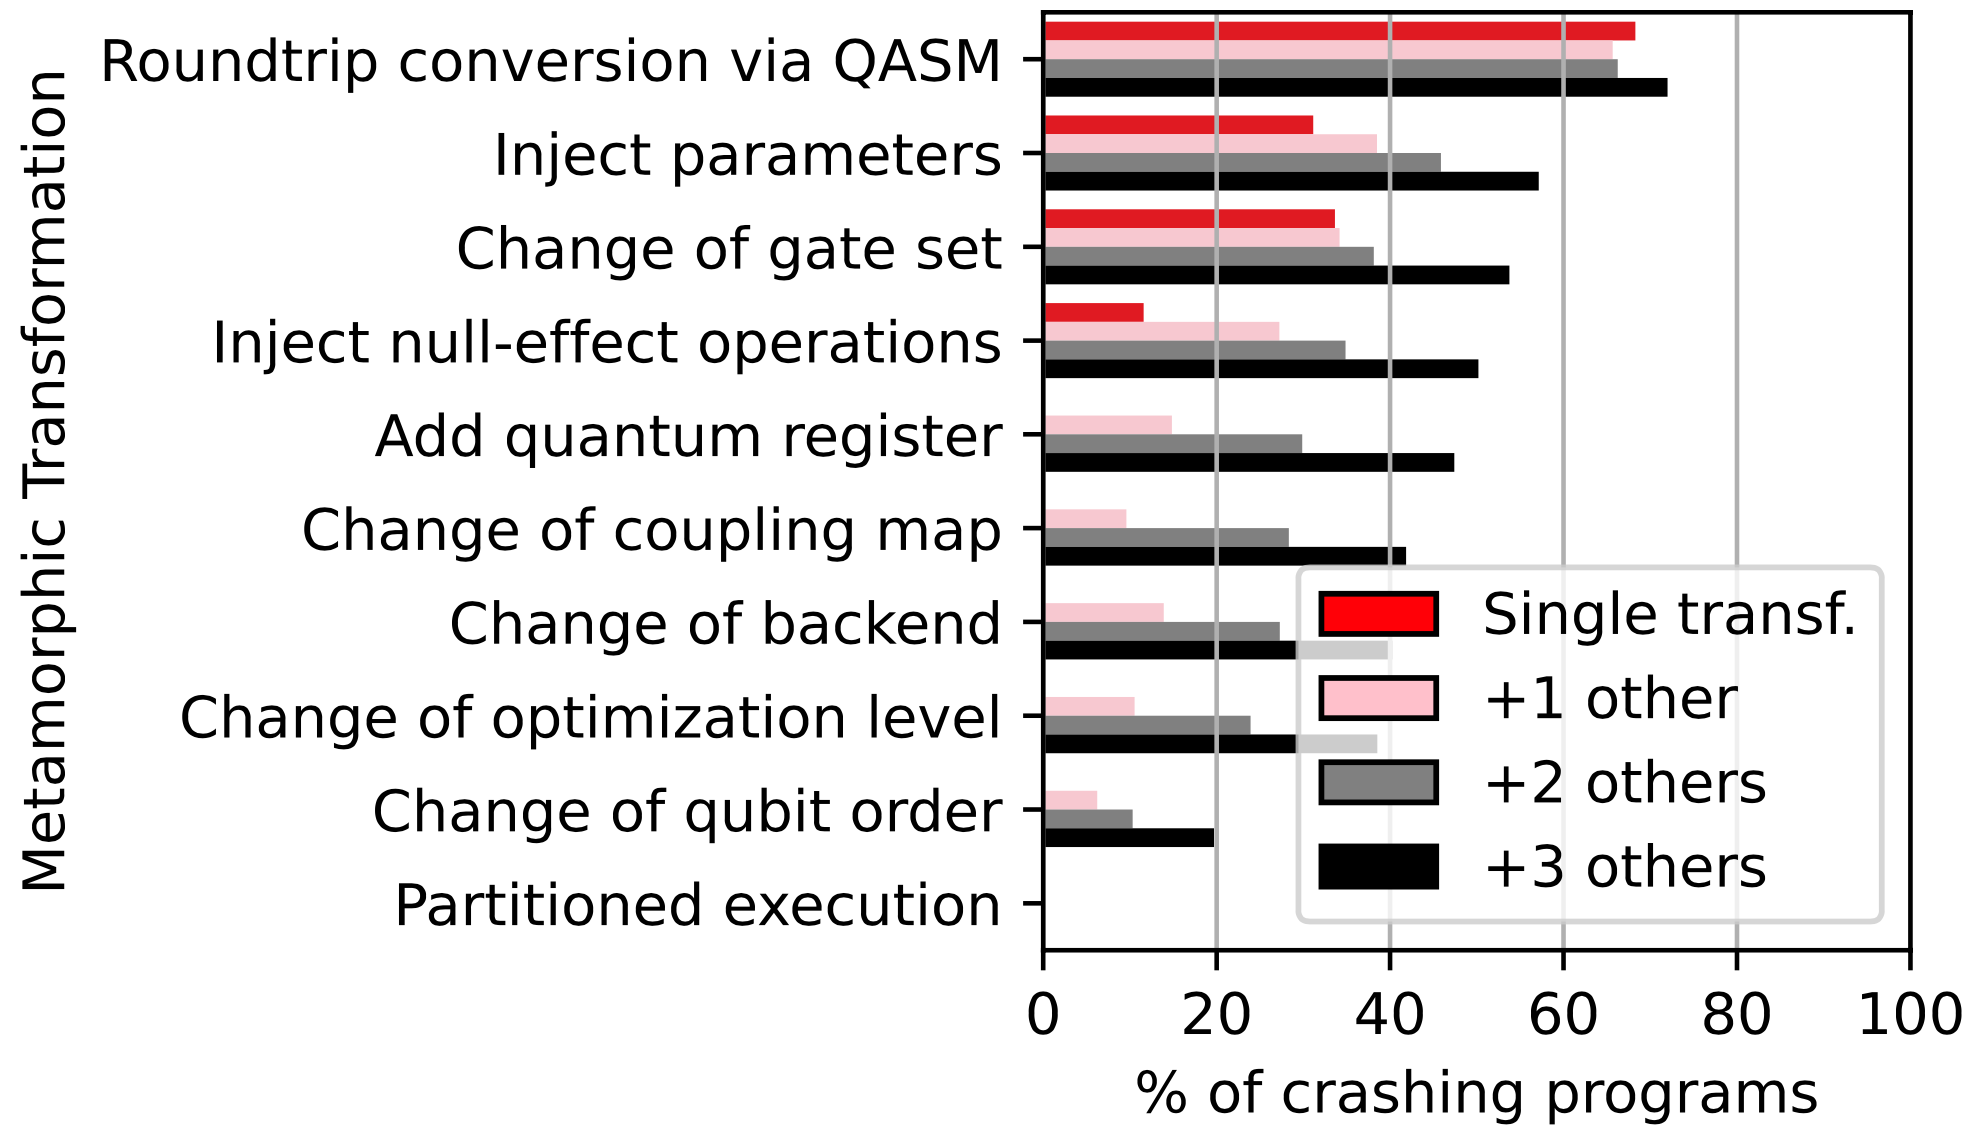
\includegraphics[width=\textwidth]{TFM/photos/MorphQMRCrash.png}
    \caption{MR analysis in follow-up QP \cite{paltenghi2023morphq}.} 
    \label{Fig:MorphQMRCrash}
  \end{minipage}
\end{figure}

\section{Quantum computing programs}
\label{Ch3.2:TQP}
After considering some of the latest results regarding testing of quantum platforms and the diverse challenges they have encountered and overcame, we will shift our focus towards testing our QP implementations. This presents a different challenge where we have an algorithm or specification and an implementation that should represent that algorithm. We will explore the recent developments and analyse different techniques used for testing an implementation (QP) of a given algorithm.

\subsection{Challenges; 25-31 May 2019}
On Testing Quantum Programs \cite{miranskyy2019testing}. Discusses complexity within Quantum computing and complexity needed to elaborate verification and validation on QPs.

\vspace{15pt}
\subsection{Assertions; 22 June 2019}
Yipeng Huang and Margaret Martonosi presented this paper in 2019, under the tittle: \textit{"Statistical assertions for validating patterns and finding bugs in quantum programs"} \cite{huang2019statistical}. The authors present the idea of using assertions to debug quantum algorithms, they classify them on classical, superposition and entanglement assertions. They will use chi-square test to compare distribution if needed.\newline

The authors propose a test case with Shor's algorithm. They are going to study different components of the algorithm such as QFT or multiplication subroutines inside of QFT doing unit testing. They quickly overview Grover's search algorithm, and how they can reverse the computations to check assertions. [Deep read needed]

\vspace{15pt}
\subsection{Runtime Assertions; 01 July-Dec 2019}
Quantum Circuits for Dynamic Runtime Assertions in Quantum Computation \cite{zhou2019quantum}. 2020 version \cite{liu2020quantum}.

\vspace{15pt}
\subsection{Model-Based testing for QP; 2020}
Quantum Software Testing \cite{usaola2020quantum}

\vspace{15pt}
\subsection{QSharpCheck; 25 September 2020}
\label{Ch3.2.1:QSharpCheck}
The initial approach we will discuss was presented by S. Honarvar et al. in 2020 with the title: "\textit{Property-based Testing of Quantum Programs in $Q\#$}" \cite{honarvar2020property}. The authors position this approach as the first step towards structured testing techniques for quantum programs, offering a property-based framework tailored for $Q\#$. Their work was influenced by Quantum Hoare Logic \cite{ying2012floyd} and assertion language \cite{huang2019statistical}. The authors introduce a syntax for specifying properties of $Q\#$ programs along with a tool named QSharpCheck, designed for test case generation, text execution, and analysis of outcomes.\newline

Let's delve into the syntax introduced for property specification. This involves associating a test property with a name and parameters, followed by allocation and setup, function call and finally assertion. This structured syntax is illustrated in Figure \ref{Fig:QSharpSyntax}, and an example is provided in Figure \ref{Fig:QSharpSyntaxEx}.

\vspace{15pt}

\begin{figure}[H]
        \centering
        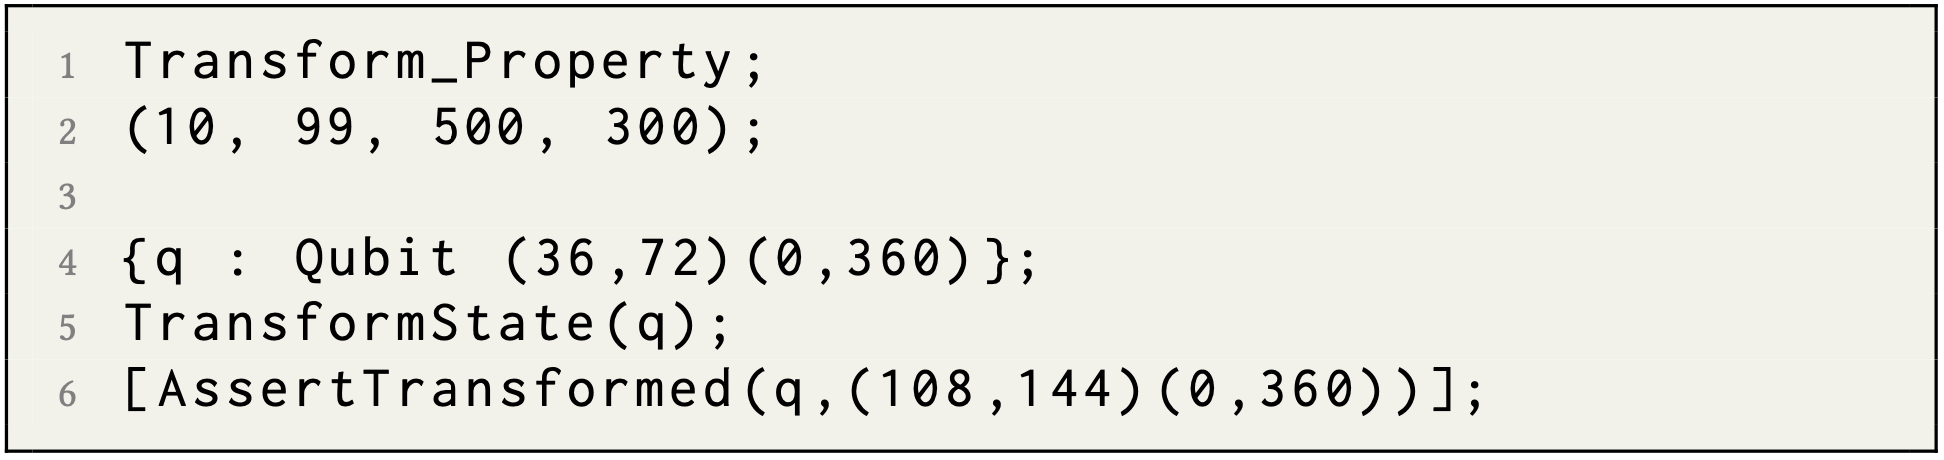
\includegraphics[width=0.5\textwidth]{TFM/photos/QsharpSyntaxEx.png}
        \caption{Property example, state transformation \cite{honarvar2020property}.} 
        \label{Fig:QSharpSyntaxEx}
\end{figure}

\begin{figure}[H]
        \centering
        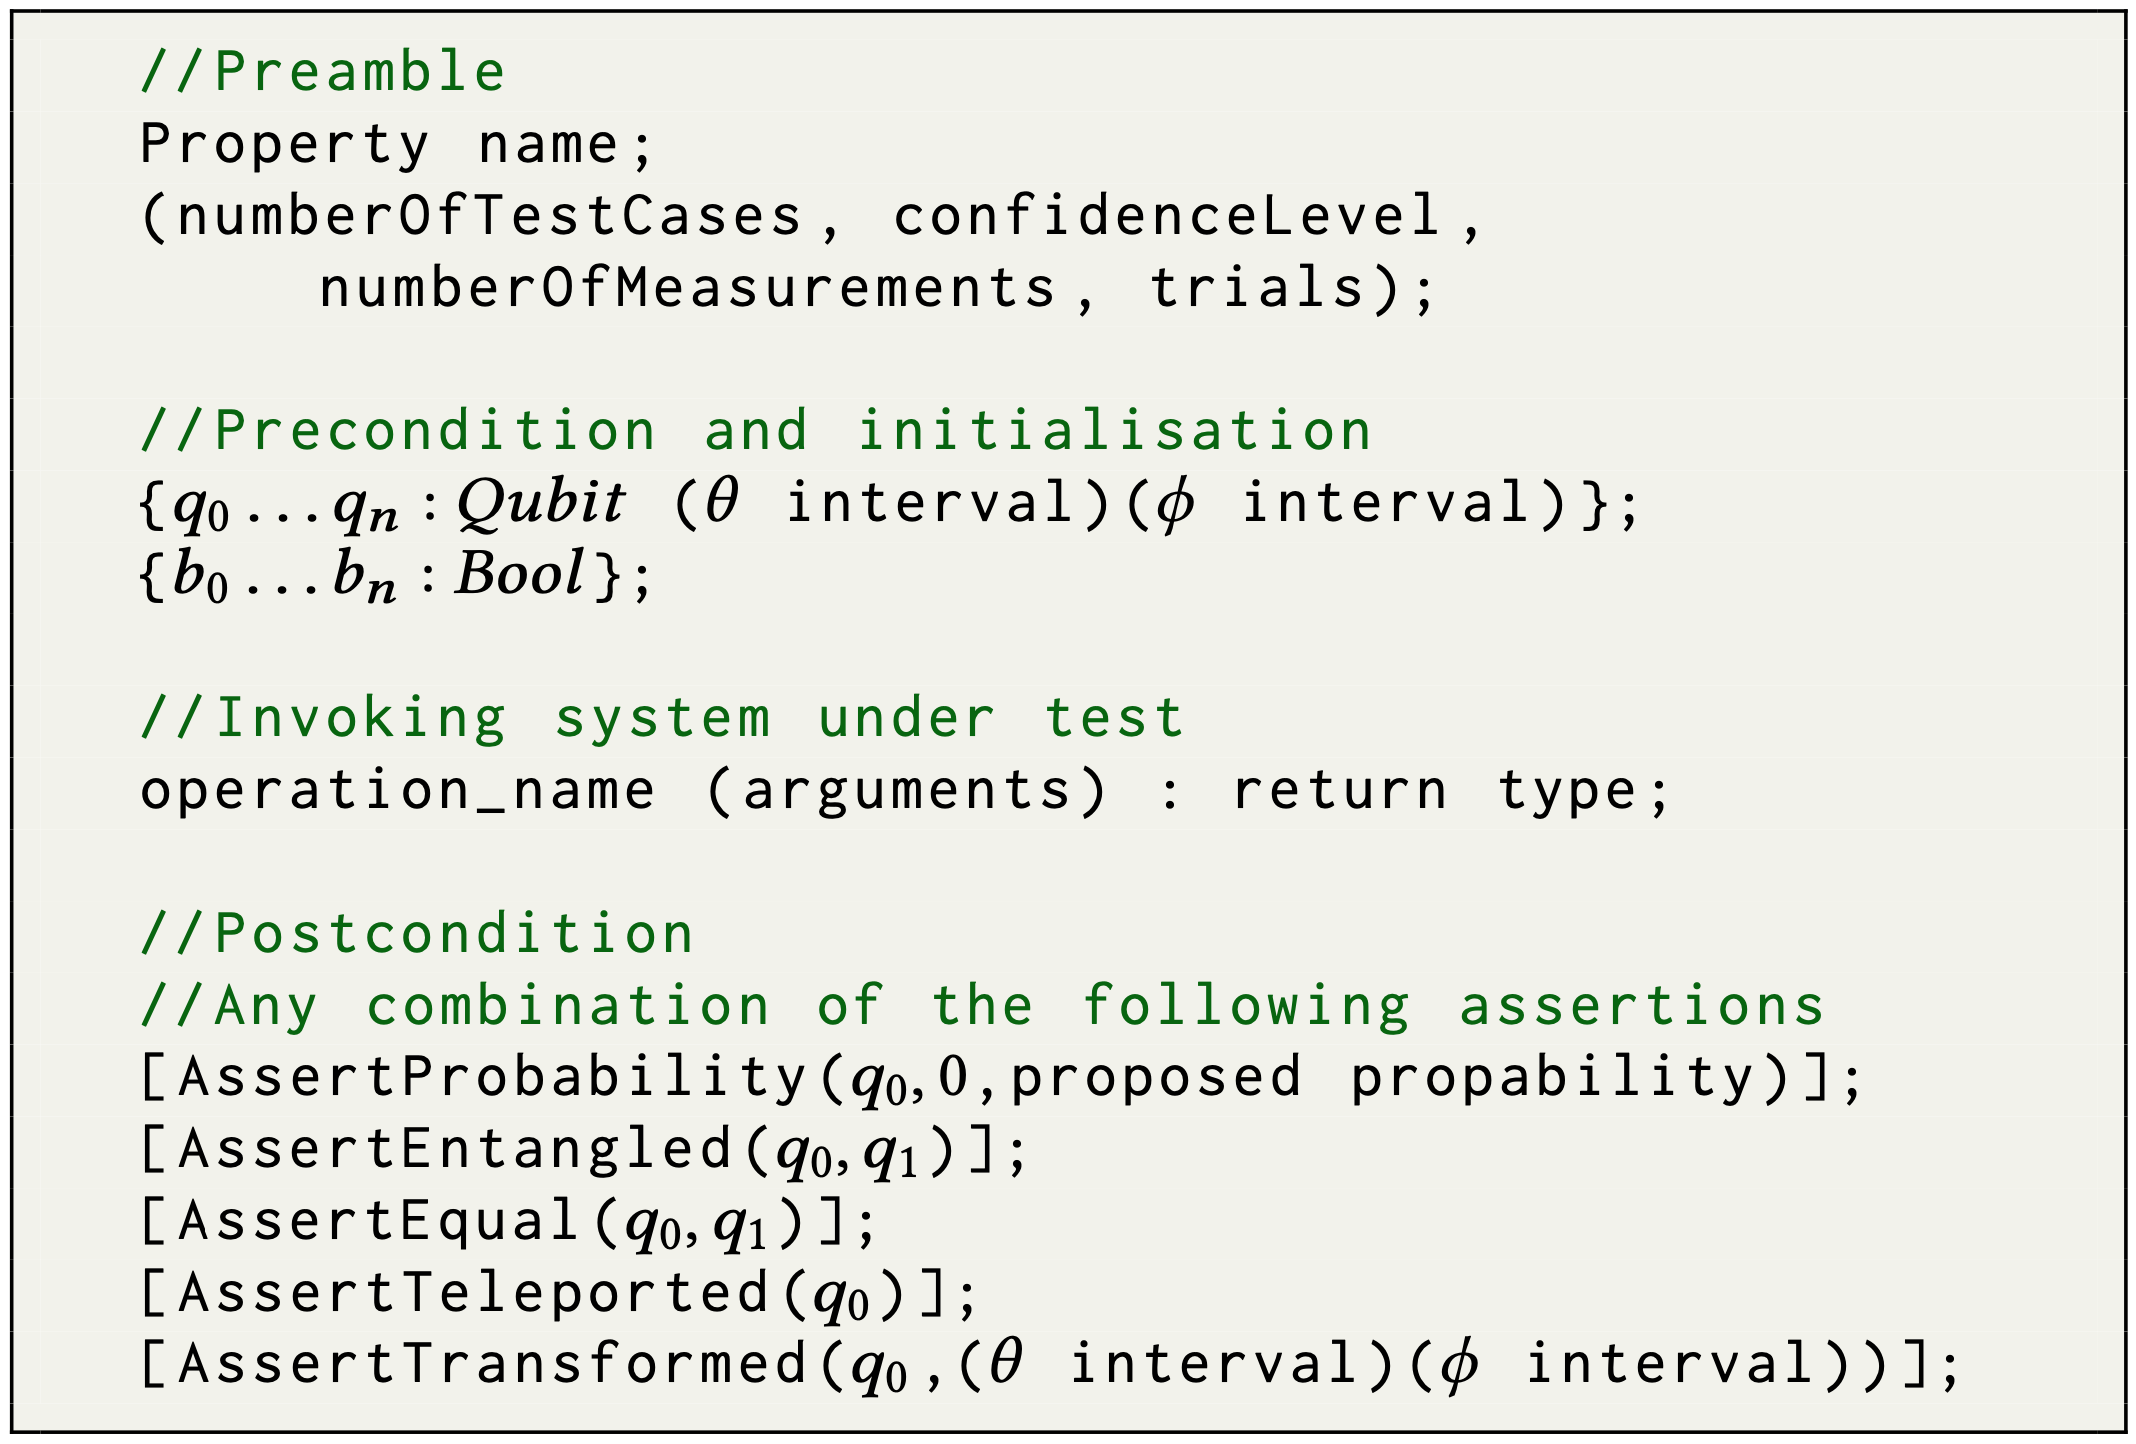
\includegraphics[width=0.5\textwidth]{TFM/photos/QsharpSyntax.png}
        \caption{Property syntax structure \cite{honarvar2020property}.} 
        \label{Fig:QSharpSyntax}
\end{figure}


With the established syntax, we can now introduce QSharpCheck, illustrated in Figure \ref{Fig:QSharpArch}. We could observe some output examples in Figure \ref{FIG:QSharpOutput}:

\begin{itemize}
    \item Test case generator. QSharpCheck functions as a test case generator, producing the specified number of test cases randomly within the range specified in the parameters.
    \item Test execution Engine. This component repeats the execution as many times as required by the specification.
    \item Statistical Analysis Engine. QSharpCheck incorporates a statistical analysis engine that performs hypothesis testing, considering the last assertion in the test as the null hypothesis. It assumes the program follows a binomial distribution, and in cases where the user doesn't provide a confidence level, it defaults to 0.99.
\end{itemize}

\begin{figure}[H]
        \centering
        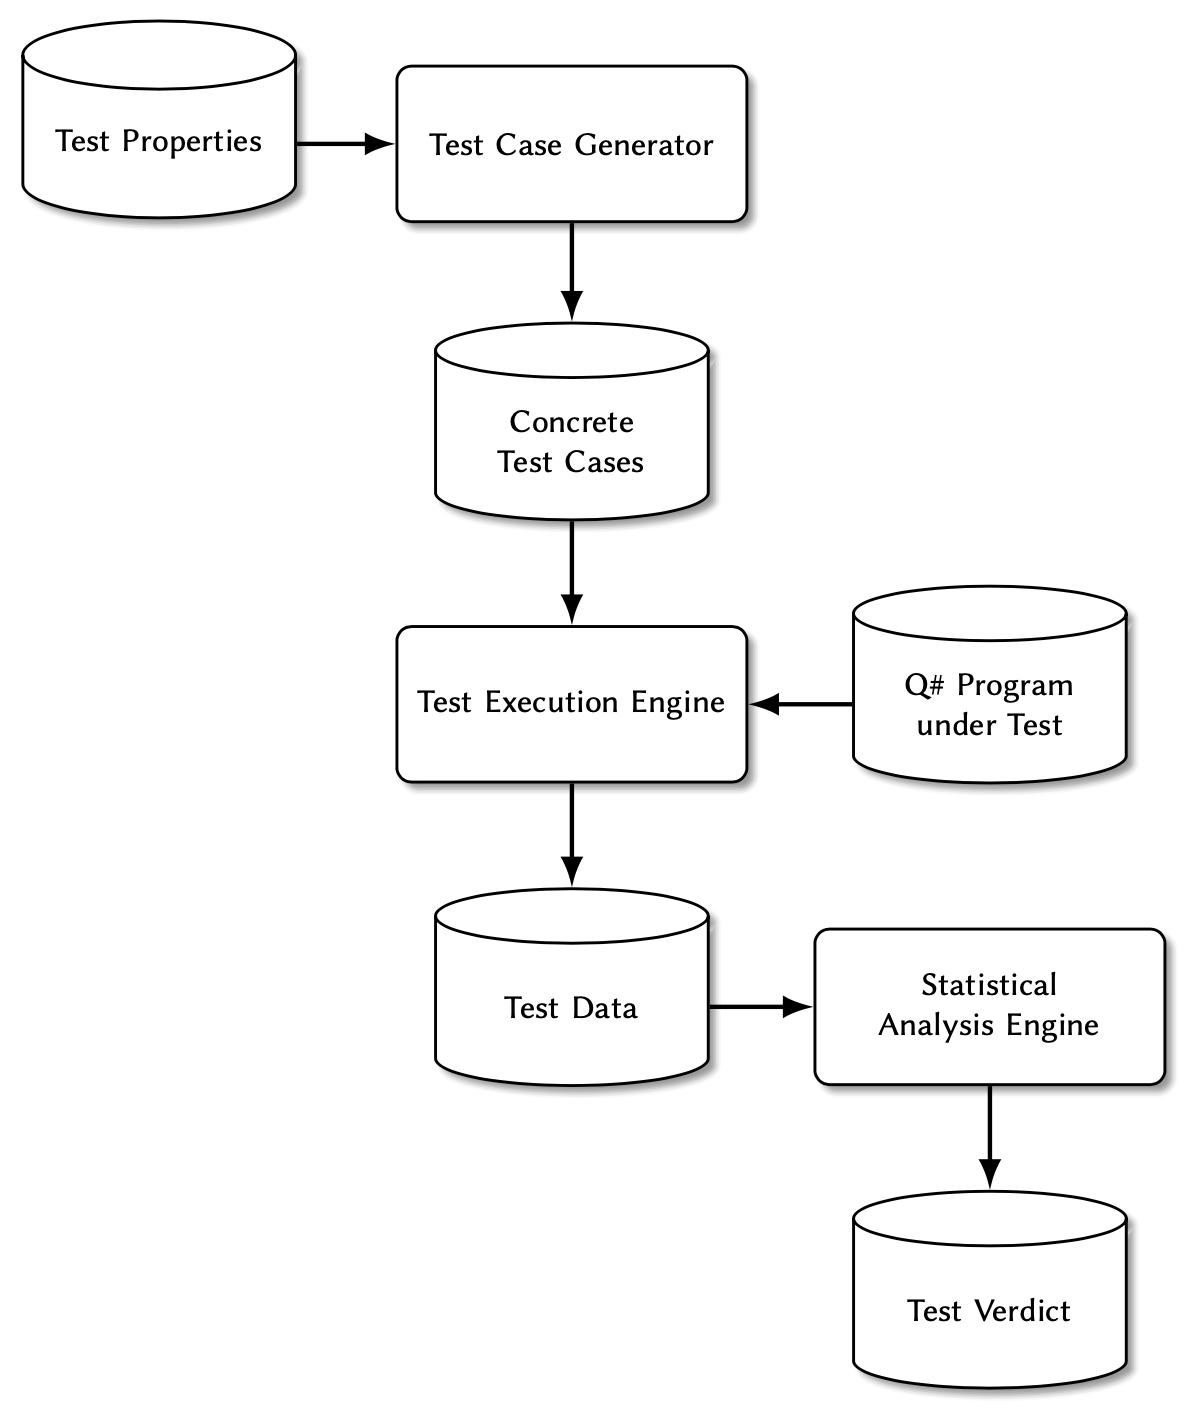
\includegraphics[width=0.4\textwidth]{TFM/photos/QSharpOverview.png}
        \caption{QSharpCheck architecture \cite{honarvar2020property}.} 
        \label{Fig:QSharpArch}
\end{figure}

\begin{figure}[H]
    \centering
    \begin{subfigure}[H]{0.48\textwidth}
        \centering
        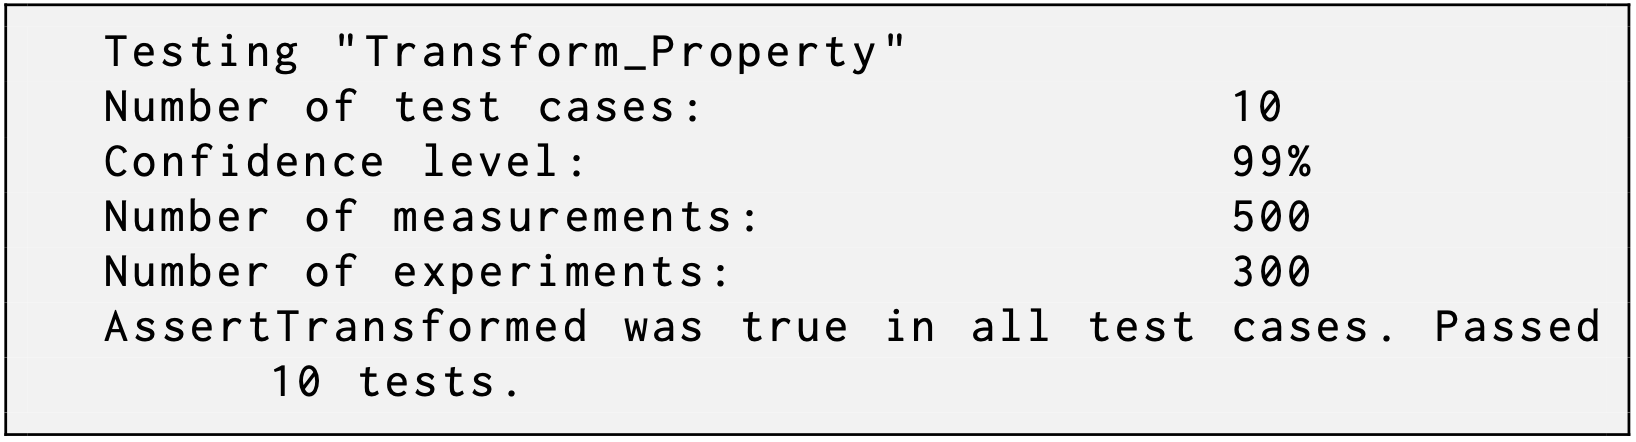
\includegraphics[width=\textwidth]{TFM/photos/QSharpOut1.png}
        \caption{QSharpCheck positive outcome.} 
        \label{Fig:QSharpOutput1}
    \end{subfigure}
    \hfill
    \begin{subfigure}[H]{0.48\textwidth}
        \centering
        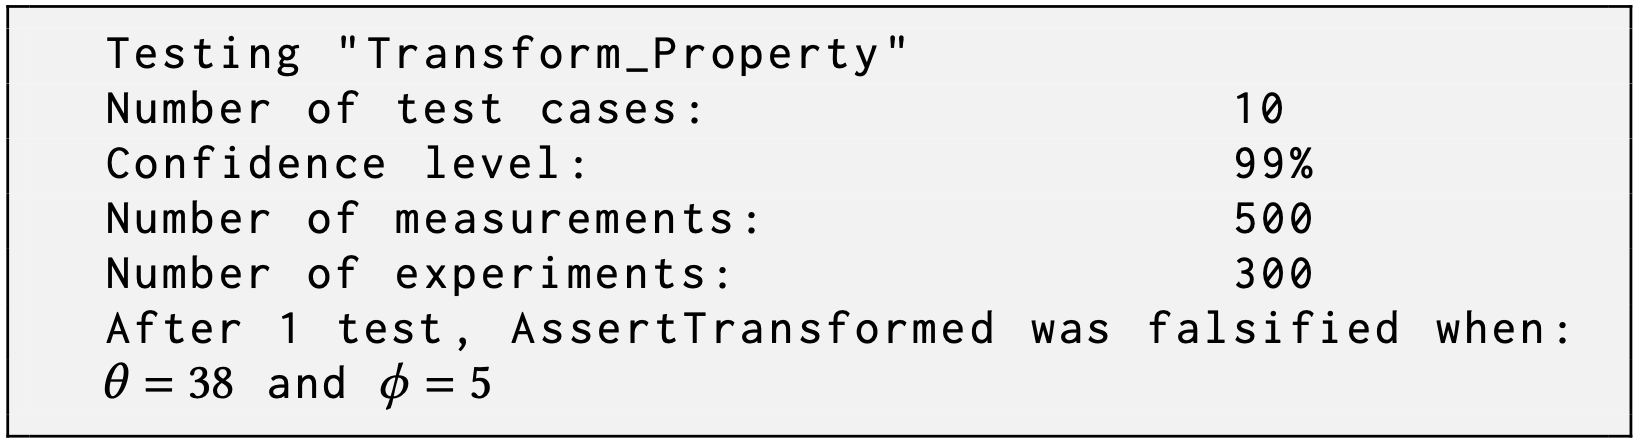
\includegraphics[width=\textwidth]{TFM/photos/Qsharpout2.png}
        \caption{QSharpCheck negative test.} 
        \label{Fig:QSharpOutput2}
    \end{subfigure}
        \caption{Two possible QSharpCheck outcomes \cite{honarvar2020property}. }
    \label{FIG:QSharpOutput}
 \end{figure}

The authors have designed QSharpCheck to accommodate various types of assertions as methods. Let's explore the types of assertions that can be used within this tool.

\begin{itemize}
    \item AssertProbability. This assertion observes if a given qubit can reach a specified measurement with a designated probability.
    \item AssertEntangled. Given two qubits as input, this assertion tests whether or not they are entangled.
    \item AssertEqual. As the name suggests, this assertion checks whether two qubits are equal. The null hypothesis is defined based on the equality of the qubits.
    \item AssertTeleported. Specifically designed for testing teleportation, this method takes the sent and received qubits as arguments. It analyses the probability found on the sent qubit and executes the \textit{AssertProbability} on the received qubit.
    \item AssertTransformed, This assertion is employed for unitary transformations.
\end{itemize}

To asses the capabilities of this framework, the authors introduce mutation testing to two programs, teleportation and superdense coding. The results yielded a mutation score of $80\%$ for teleportation and $60\%$ for superdense coding, with 20 mutant programs examined in each case.\newline

The authors conclude the article by summarising the completed work, emphasising that this marks the initial phase in property-based testing of QPs. The primary contribution of the article lies in the integration of a property language based on pre- and post-condition type properties and QSharpCheck.

\vspace{15pt}
\subsection{Proq; 13 November 2020}

Projection-based runtime assertions for testing and debugging Quantum programs \cite{li2020projection}

\vspace{15pt}
\subsection{QCEC; February 2021*}

Bulgholzer et al. presented in 2021 the tool QCEC in the paper with title: \textit{QCEC: A JKQ tool for quantum circuit equivalence checking} \cite{burgholzer2021qcec}. The authors present QCEC as an equivalent checker tool developed in C++ as part of JKQ toolset although they presented the binding for python users.\newline

The idea behind this method is that quantum programs are reversible if measurement has not taken place, therefore we can compute the inverse and check if the product produce the identity matrix. The methods implemented in QCEC, which will be summarised in Figure \ref{Fig:QCEC}, were presented previously in their papers \cite{burgholzer2020improved}\cite{burgholzer2020power}\cite{niemann2015qmdds}\cite{burgholzer2020verifying}\cite{burgholzer2021random}. The authors conclude that due to the generality of the tool, it could be specified for an specific scenario and even incorporated to other languages.

\begin{figure}[H]
        \centering
        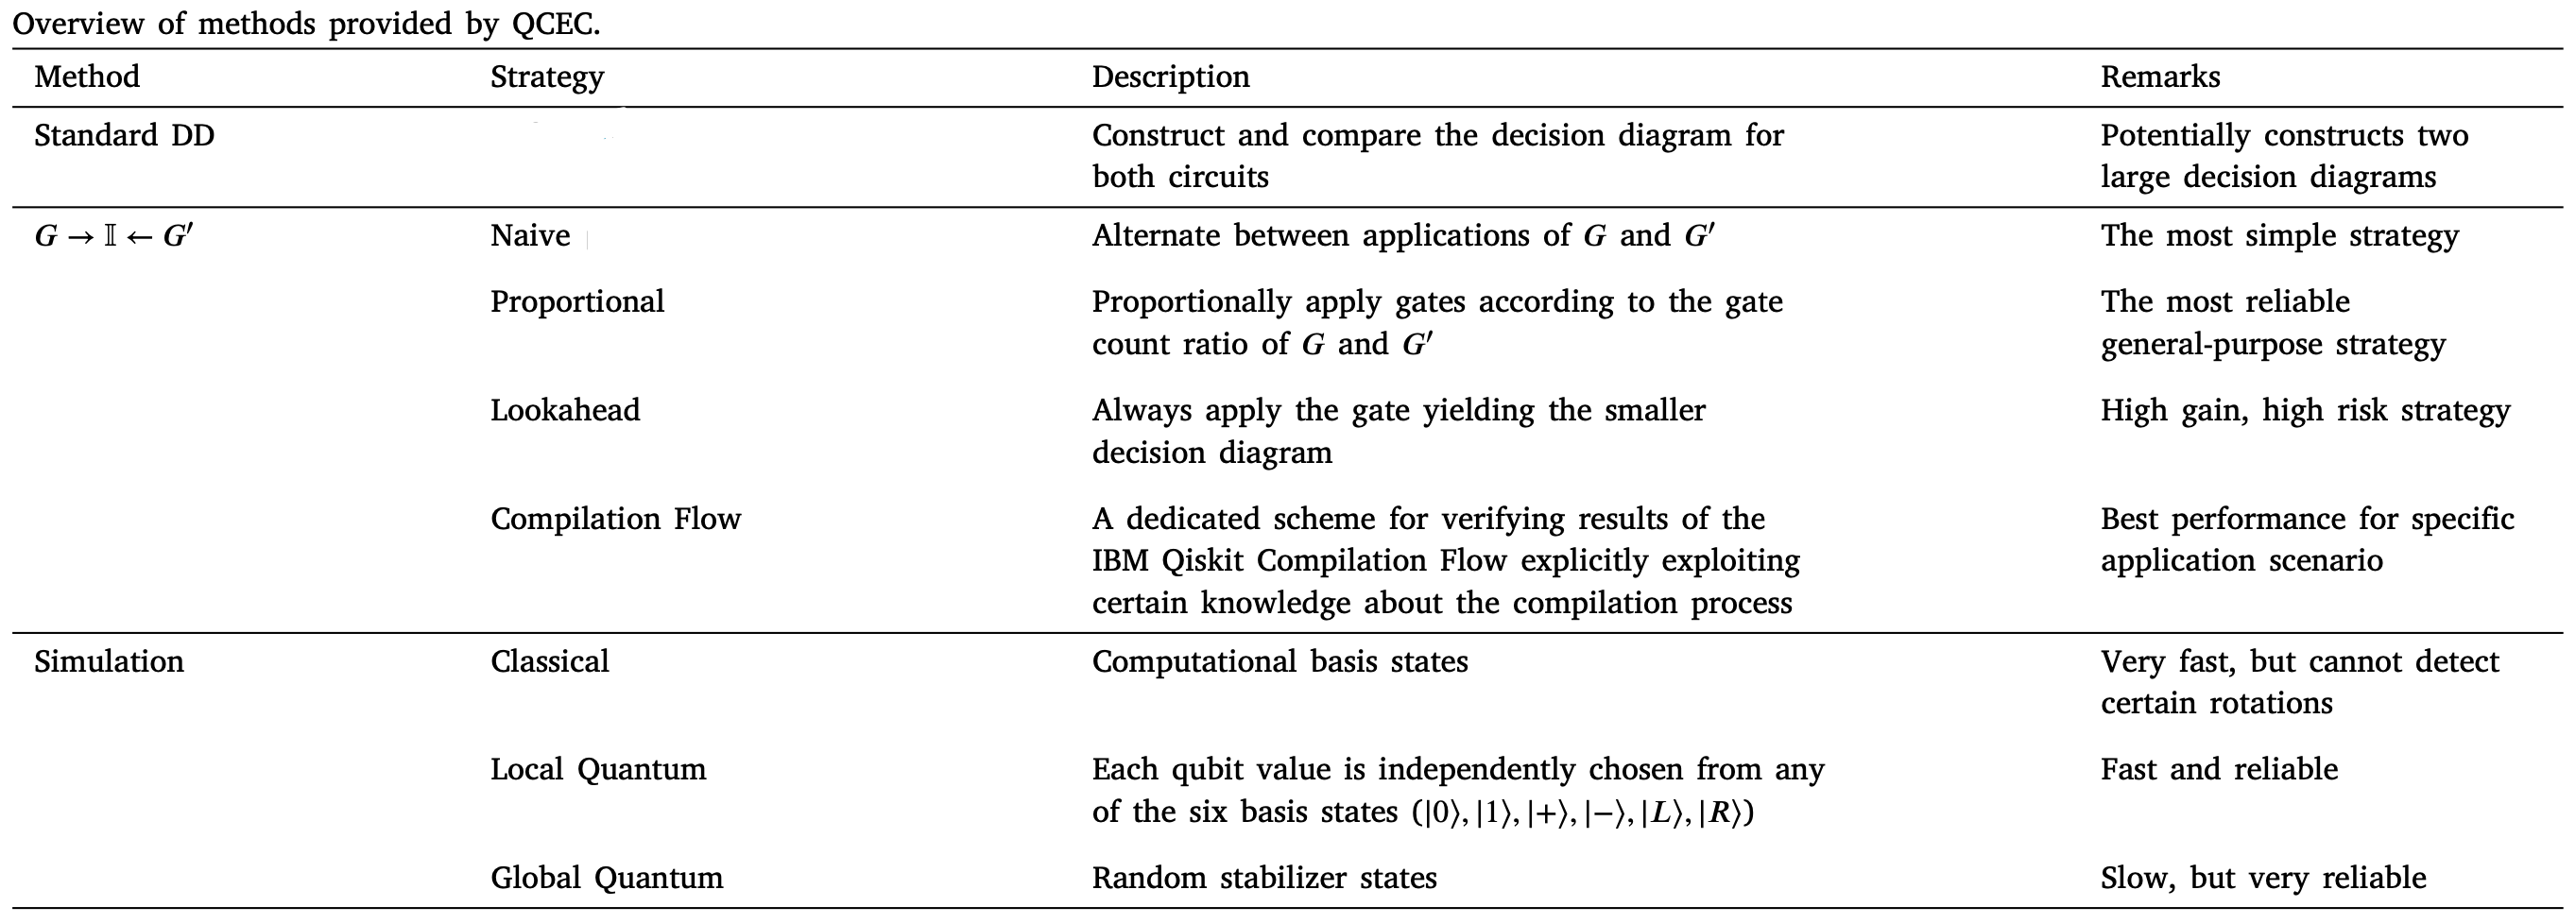
\includegraphics[width=0.4\textwidth]{TFM/photos/QCEC.png}
        \caption{QCEC methods \cite{burgholzer2021qcec}.} 
        \label{Fig:QCEC}
\end{figure}

\vspace{15pt}
\subsection{QuanFuzz; 12-16 April 2021 W}

Check! First article on 16 Oct 2018 \cite{wang2018quanfuzz}
Poster: Fuzz Testing of Quantum Program 
 \cite{wang2021poster}

\vspace{15pt}
\subsection{Quito; 12-16 April 2021}
\label{Ch3.2.2:Quito}

 The subsequent approach, presented by S. Ali et all in 2021 under the title: "\textit{Assessing the effectiveness of input and output coverage criteria for testing quantum programs}"\cite{ali2021assessing}, introduces the Quito approach (QUantum InpuT Output coverage). The authors define three coverage criteria on the inputs and outputs of QPs along with their test generation strategies. This paper has been expanded to include new experiments, as detailed in \cite{wang2021quito}.\newline

In their paper, the authors formally establish definitions for QP, input, output, program specification, valid output values, and test input, output, and suite. As well, the definition of input, output and input-output criteria follows the usual such that every input/output/<input,output>, respectively,  is covered by a test suite. Let's delve in their definition for outcome of a test suite:

\vspace{8pt}
\begin{itemize}
    \item Definitely fail: The outcome returns a non-valid output.
    \item Likely fail: The tested probability significantly deviates from the expected probability based on the Wilcoxon test with a $99\%$ confidence interval.
    \item Inconclusive: No failure has been detected.
\end{itemize}

To proceed, the authors propose the application of two different oracles in sequence:

\vspace{-3pt}
\begin{itemize}
    \item Wrong Output Oracle, WOO: Checks if QP only produces valid output values.
    \item Output Probability Oracle, OPO: Verifies if the QP returns an expected output with its associated probability. Providing one of the outcomes explained previously.
\end{itemize}

Let us introduce the test suit generators for testing.To initiate the process, the user will define a parameter $K$ representing the desired number of test suites. Additionally, a budget for output coverage need to be allocates as a constraint for generating a single test suite, because there is a chance of not finding the correct input for a particular output. The test suite creation algorithms will directly assess the WOO, halting if a non-valid output is produced and saving that test suite as a WOO failure.

\vspace{-3pt}
\begin{itemize}
    \item Input coverage. For each value up to $K$, each possible input will be executed and saved if it produces a valid output.
    \item Output coverage. For each value up to $K$, while there is elements in the valid outputs set and our budget for a single test suite generation has not been exhausted:
    \begin{itemize}
        \item[-] Execute one element from the valid input set.
        \item[-] Add $\langle$input, output$\rangle$ to the test suite.
        \item[-] Remove the output from the valid outputs set.
    \end{itemize}
    \item Input-Output coverage. For each value up to $K$ and for each valid input, we define the valid outputs set from the specification and proceed similarly to output coverage with this set and budget.
\end{itemize}

Therefore, we can now outline the Quito workflow:
\begin{itemize}
    \item Test suites generation.
    \item Check for WOO outcomes, already evaluated during test suite creation. The outcome will be \textit{definitely fail} if fails WOO.
    \item For test suites that pass WOO, they will be assessed by OPO. Since larger test suites may be required for statistical significance, it may be necessary to merge some test suites to meet this criterion. The outcome will be either \textit{likely fail} or \textit{inconclusive}.
\end{itemize}

The authors intend to assess these coverage criteria using mutation analysis, employing the following categories of mutation operators: add gate (AG), delete gate (DG), replace gate (RG), and replace mathematical operator (RMO), these operator behave similarly to classical mutation operators. The effectiveness of their test suites will be evaluated on mutated programs. Since results may vary across executions, each test suite will be executed K times for each criteria.\newline

A mutant will be considered "killed" if at least one of the proposed oracles fails. The mutation score is defined by subtracting the number of equivalent mutants from the total number of mutants. As the number of equivalent mutants is initially unknown, the authors start with 0 and analyse it after testing. The equivalent mutants are then studied manually, step by step, comparing states from the original process to a mutated one using the QCEngine execution facility.\newline

Let us summarise the key results and contributions of Quito:
\begin{itemize}
    \item Three coverage criteria: Quito introduces three coverage criteria that are independent of a specific language, each equipped with its own algorithm for creating test suites to achieve full coverage.
    \item Consistent Mutation Scores: The mutation scores tend to remain within the same range regardless of the coverage criteria. Although there are some variations, achieving higher mutation scores comes with a significant computational cost. For instance, RCR reaches an $80\%$ mutation score with 8000 test cases in input coverage and over 15000 in output coverage. However, it attains a $95\%$ mutation score on input-output coverage but requires 160k test cases.
    \item Equivalent Mutants: All non-killed mutants were identified as equivalent mutants, and some exhibited a phase difference.
\end{itemize}

To conclude this approach, let's consider some potential future work that is either underway or could be explored:

\begin{itemize}
    \item Testing QP phases: To obtain a reduction of test cases through boundary values and equivalence partitioning.
    \item There is no knowledge/approach about equivalent mutants in QP.
    \item There is no knowledge/guide regarding the appropriate setup of parameters for these coverage criteria.
\end{itemize}

\vspace{15pt}
\subsection{QuSBT; 29 September 2021 W}

Generating Failing Test Suites for Quantum Programs With Search \cite{wang2021generating}

2022 version \cite{wang2022qusbt}

\vspace{15pt}
\subsection{Testing QSharp with Microsoft development kit; October 19, 2021*}

Mykhailova et al. presented the papaer with tittle: \textit{Testing Quantum Programs using Q$\#$ and Microsoft Quantum
Development Kit} \cite{mykhailova2021testing}, where the authors present Q$\#$ and using the open-source QDK shows how testing could be implemented. The key contribution is the small examples where it grows from unit testing to unitary transformations using Katas \cite{mykhailova2020quantum}, which is a tutorial with feedback, and applying Choi-Jamiolkowski isomorphism \cite{choi1975completely}\cite{jamiolkowski1972linear} to simplify checks.

\vspace{15pt}
\subsection{Muskit; 15-19 November 2021}
\label{Ch3.2.3:Muskit}
The third approach was introduced by E. Mendiluze et al. with the title: "\textit{Muskit: A Mutation Analysis Tool for Quantum Software Testing}"\cite{mendiluze2021muskit} in 2021. The authors present Muskit as the novel tool to autonomously implement mutation testing in Quantum Programs (QPs). While there were some previous works\cite{ali2021assessing}\cite{wang2021quito} utilising mutation testing in quantum, all mutated programs were manually generated.\newline

As evident from the Muskit architecture (Figure \ref{Fig:MuskitArch}), Muskit comprises two main components, with the added Test Analyser. Let's delve into these components. The first, and a key result of this paper, is the introduction of a mutation generator. Let's explore the various mutation operators employed and the criteria the tool uses to implement them.

\begin{figure}[H]
        \centering
        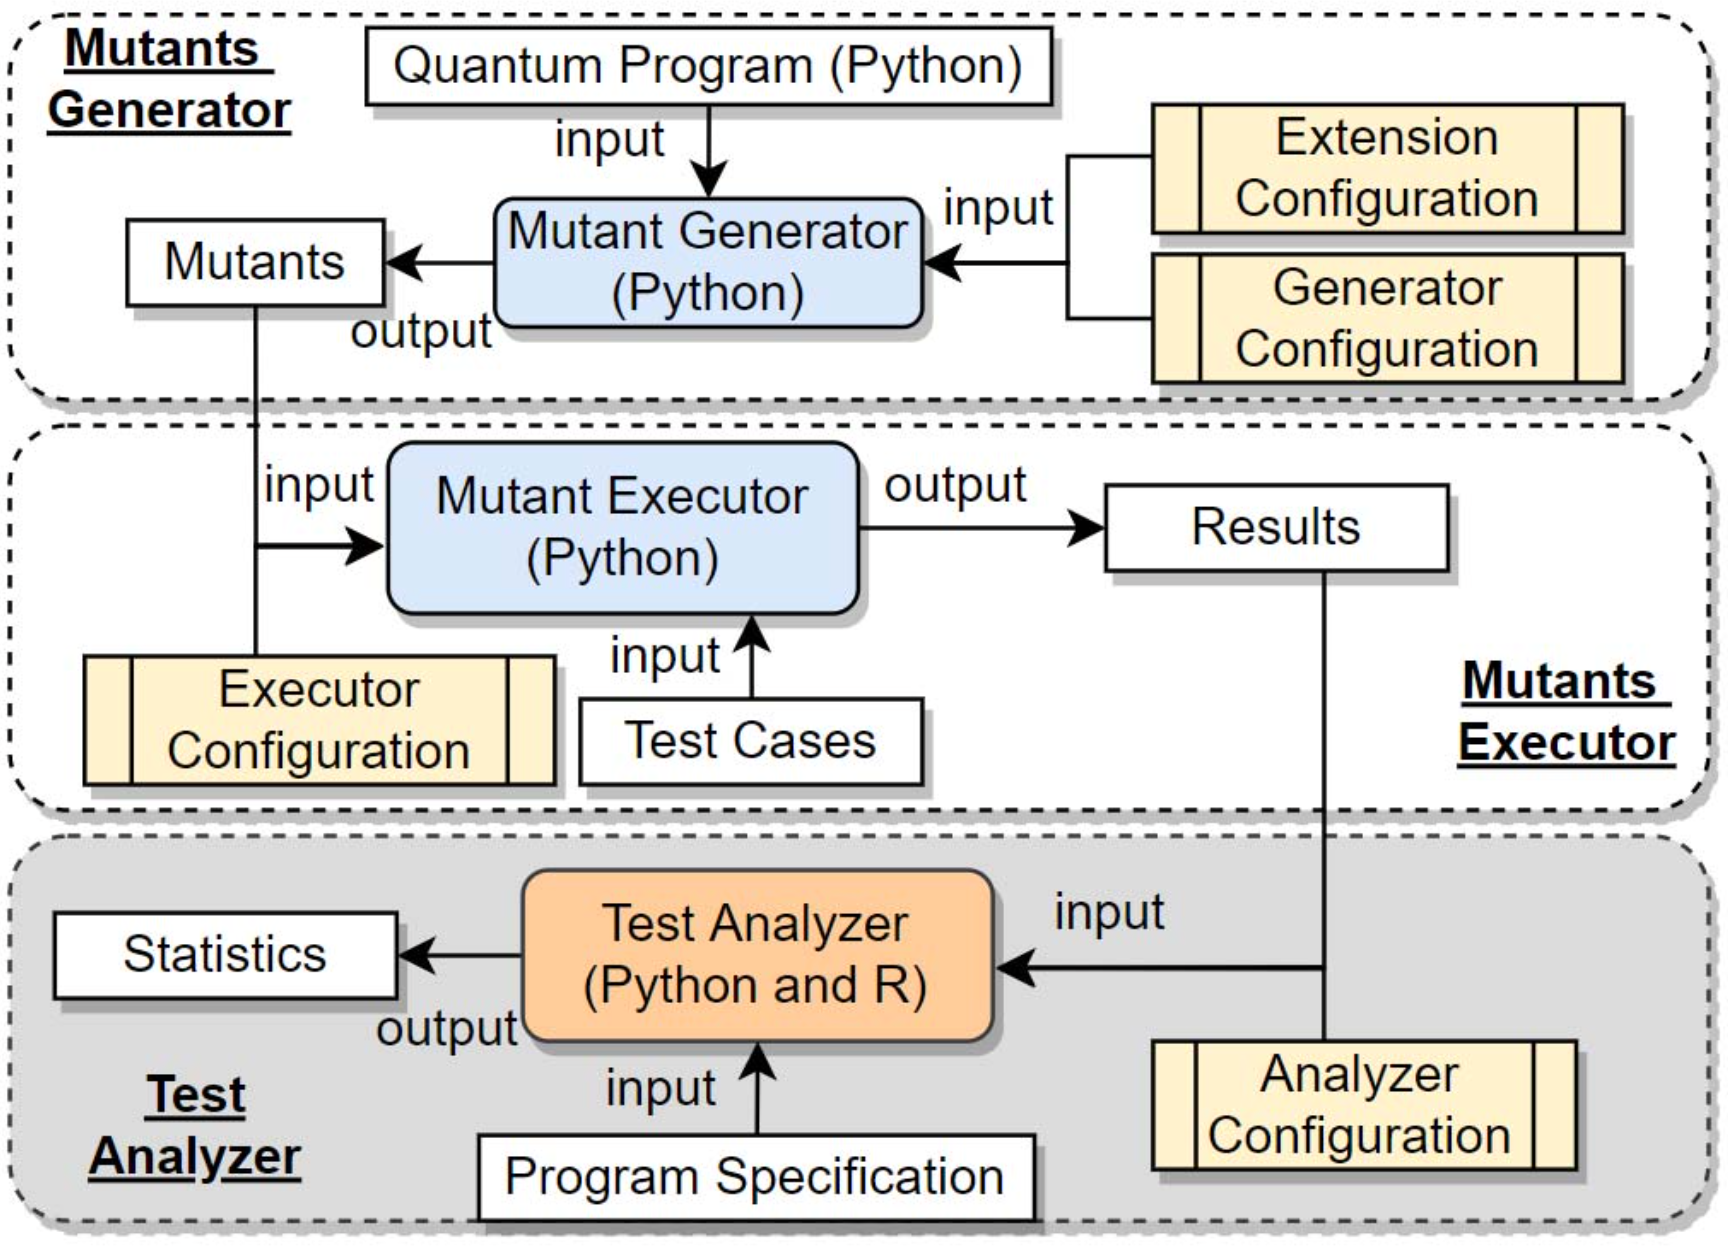
\includegraphics[width=0.46\textwidth]{TFM/photos/MuskitOverview.png}
        \caption{Muskit architecture \cite{mendiluze2021muskit}} 
        \label{Fig:MuskitArch}
\end{figure}

Mutation operators supported for 19 gates:
\begin{itemize}
    \item Add Gate (AG).
    \item Remove Gate (RemG).
    \item Replace Gate (RepG). Replacing an existing gate for one compatible, applied to the same number of qubits.
\end{itemize}

Mutation criteria, will reduce the number of mutants to be generated:
\begin{itemize}
    \item All. All possible mutants are generated.
    \item Operator Selections. The user has the flexibility to choose which mutant operators they would like to use.
    \item Gate Selection. The user controls mutant generation based on the number of qubits. Muskit supports three categories: one qubit gates, two qubit gates and three or more qubit gates. 
    \item Gate Number Selection. The user can control what gate will be mutated, as Muskit maps gates to numbers.
    \item Location Number. The user can locate where to apply AG.
    \item Phase Selection. The user can select a phase between 0 and 360 when mutants are applied to phase gates.
    \item Maximum Number. One can limit the number of mutants to be generated.
\end{itemize}

When focusing on the Mutants Executor component, it takes mutants and test cases as input, executing them as many times as specified in a file called \textit{ExecutorConfiguration}. In cases where no specification is provided for the input test cases, it defaults to using the \textit{Input coverage} as presented in \ref{Ch3.2.2:Quito}\cite{ali2021assessing} by S. Ali et al. The tool follows a similar approach for the Test Analyser component, importing both oracles—Wrong Output Oracle (WOO) and Output Probability Oracle (OPO)—from \ref{Ch3.2.2:Quito}\cite{ali2021assessing}. Once analysed, all results are reported.\newline

The authors conducted experiments using four different QPs to evaluate Muskit, yielding the results shown in Figure \ref{Fig:MuskitRes}, to demonstrate the capability of automatically generating mutants in QP

\begin{figure}[H]
        \centering
        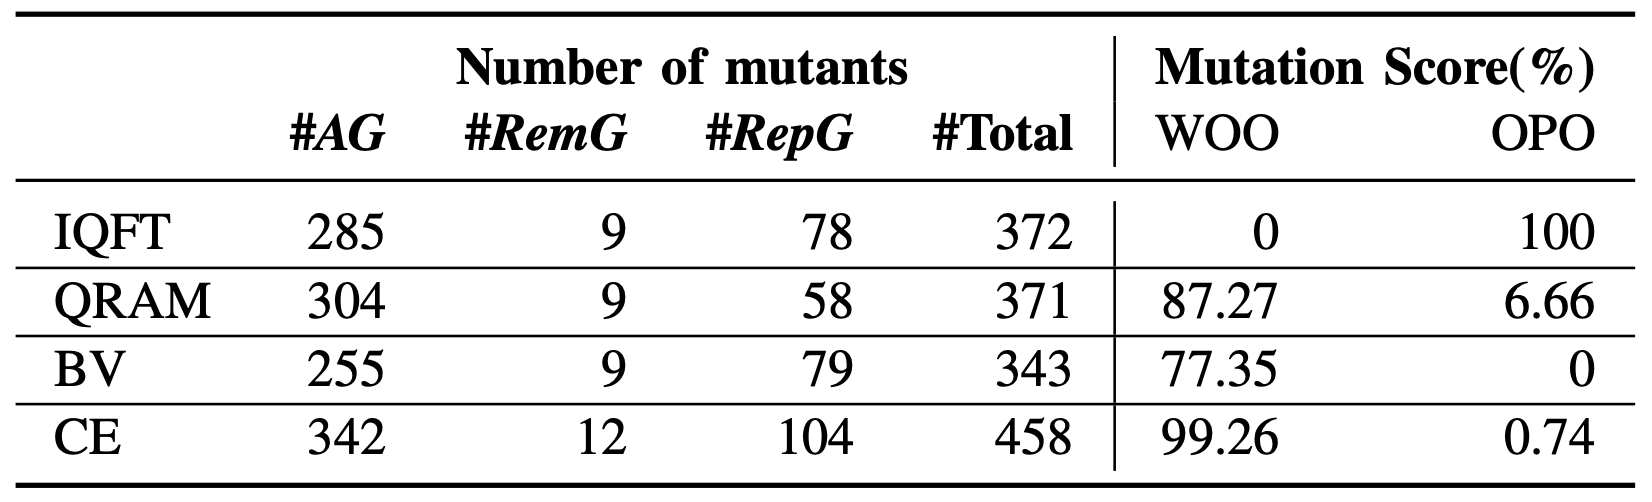
\includegraphics[width=0.7\textwidth]{TFM/photos/MuskitResults.png}
        \caption{Muskit results \cite{mendiluze2021muskit}} 
        \label{Fig:MuskitRes}
\end{figure}

. Until now, all mutations had been performed manually. The paper identifies a limitation that Muskit currently faces, it is unable to detect equivalent mutants. The authors express concerns about the possibility that these quantum mutation operators may be related to each other in terms of the killability of their mutants. This leaves room for exploration in theoretical and experimental future works, presenting an area that could be further investigated.

\vspace{15pt}
\subsection{QuCat; 06-10 December 2021*}

Wang et al. presented \textit{Application of Combinatorial Testing to Quantum Programs} \cite{wang2021application} in 2021, where they propose an approach called QuCAT for systematic and automated testing. The main definitions are the usual defined for Wang et al. as we could see them defined on "Ref generation needed for subsec".\newline

QuCAT generates combinatorial test suites using different generation algorithms such as AETG 19 \cite{cohen1997aetg}, IPO 20 \cite{lei1998parameter}, IPOG \cite{lei2007ipog}. The idea for their experiments is to evaluate the effectiveness of using combinatorial testing, CT, for quantum programmes in two different scenarios, first will generate a test suite for a designated strength and then an incremental strength. To asses QuCAT the propose an experiment with 6 algorithms with injected faults. Let us see the RQ proposed by the authors and their answers:

\begin{itemize}
    \item[] \textbf{RQ1} How do applications of CT with different strengths compare to each other in terms of cost and effectiveness?
        \begin{itemize}
            \item CT with lower strength has significantly less cost, associated to the size.
            \item Their analysis shows that CT with a higher strength will be more effective, although for easy faults CT can achieve good results with a lower strength.
        \end{itemize}
    \item[] \textbf{RQ2} How is the effectiveness of CT with different strengths as compared to random testing?
        \begin{itemize}
            \item On average, CT has a higher success on fault detection that random approach for all strengths.
        \end{itemize}
    \item[] \textbf{RQ3} How quickly can CT find a fault as compared to random testing?
        \begin{itemize}
            \item CT can find faults more quickly than random, results are from scenario 2, for all faulty programs.
        \end{itemize}
\end{itemize}

The authors propose as future work the development of a fault localisation approach for quantum programs from this results. As they will keep testing this approach with more complex QP.

\vspace{15pt}
\subsection{Quantum bug fixes comprehensive study; 15-18 March 2022*}

Luo et al. presented the article with title: \textit{"A Comprehensive Study of Bug Fixes in Quantum Programs"} \cite{luo2022comprehensive}, where they collect all possible bugs they could find in GitHub, Stack Overflow and Stack Exchange about Qiskit, Q\#, Circ and ProjectQ to anylise and study the current bugs present in quantum programs and their fixes.\newline

The authors obtain the bugs and their fix from the cited platforms, then they filter them by three criteria they chosen: related to quantum program, written by developers and valid pre- and post-fixing codes. Once all this capturing and treatment information is done, they proceed to anylise the different bugs. Their aim is to collect all possible information and categorise it by different approaches, the first one was defined by Zhong and Su in \cite{zhong2015empirical} about fault complexity and then one based on Paltenghi and Pradel's work in \cite{paltenghi2022bugs} which clasifies bug patterns. This way they are able to answer their research questions with their findings.

\begin{itemize}
    \item[] \textbf{RQ1} Does this bug only occur in quantum programs?
        \begin{itemize}
            \item The number of quantum-specific bugs (Above 80$\%$) is much greater that the number of classical bugs.
        \end{itemize}
        
    \item[] \textbf{RQ2} Where is the location of the bug in the programs?
        \begin{itemize}
            \item All bugs have been fixed within their source file. This may be misleading, as most of the programs only had the source file.
            \item Over 70$\%$ of bugs can be fixed modifying one line of code.
        \end{itemize}
        
    \item[] \textbf{RQ3} How complex to fix bugs in quantum programs?
        \begin{itemize}
            \item Since single lines fix the bug there is a higher proportion of easy fix QP.
            \item The most complex bugs are usually related to incorrect implementation method, where the user does not know exactly the correct implementation, but this get reduced with the experience of the user. The problem is that this error is difficult for a bug-fix automation approach.
        \end{itemize}
        
    \item[] \textbf{RQ4} Are there bug patterns in the quantum pro- gram?
        \begin{itemize}
            \item Bug patterns, Figure \ref{Fig:bugPatterns}.
            \item While classical bugs are more evenly distributed over all categories, quantum bugs are mainly concentrated in API-related and math-related.
        \end{itemize}
\end{itemize}

\begin{figure}[H]
        \centering
        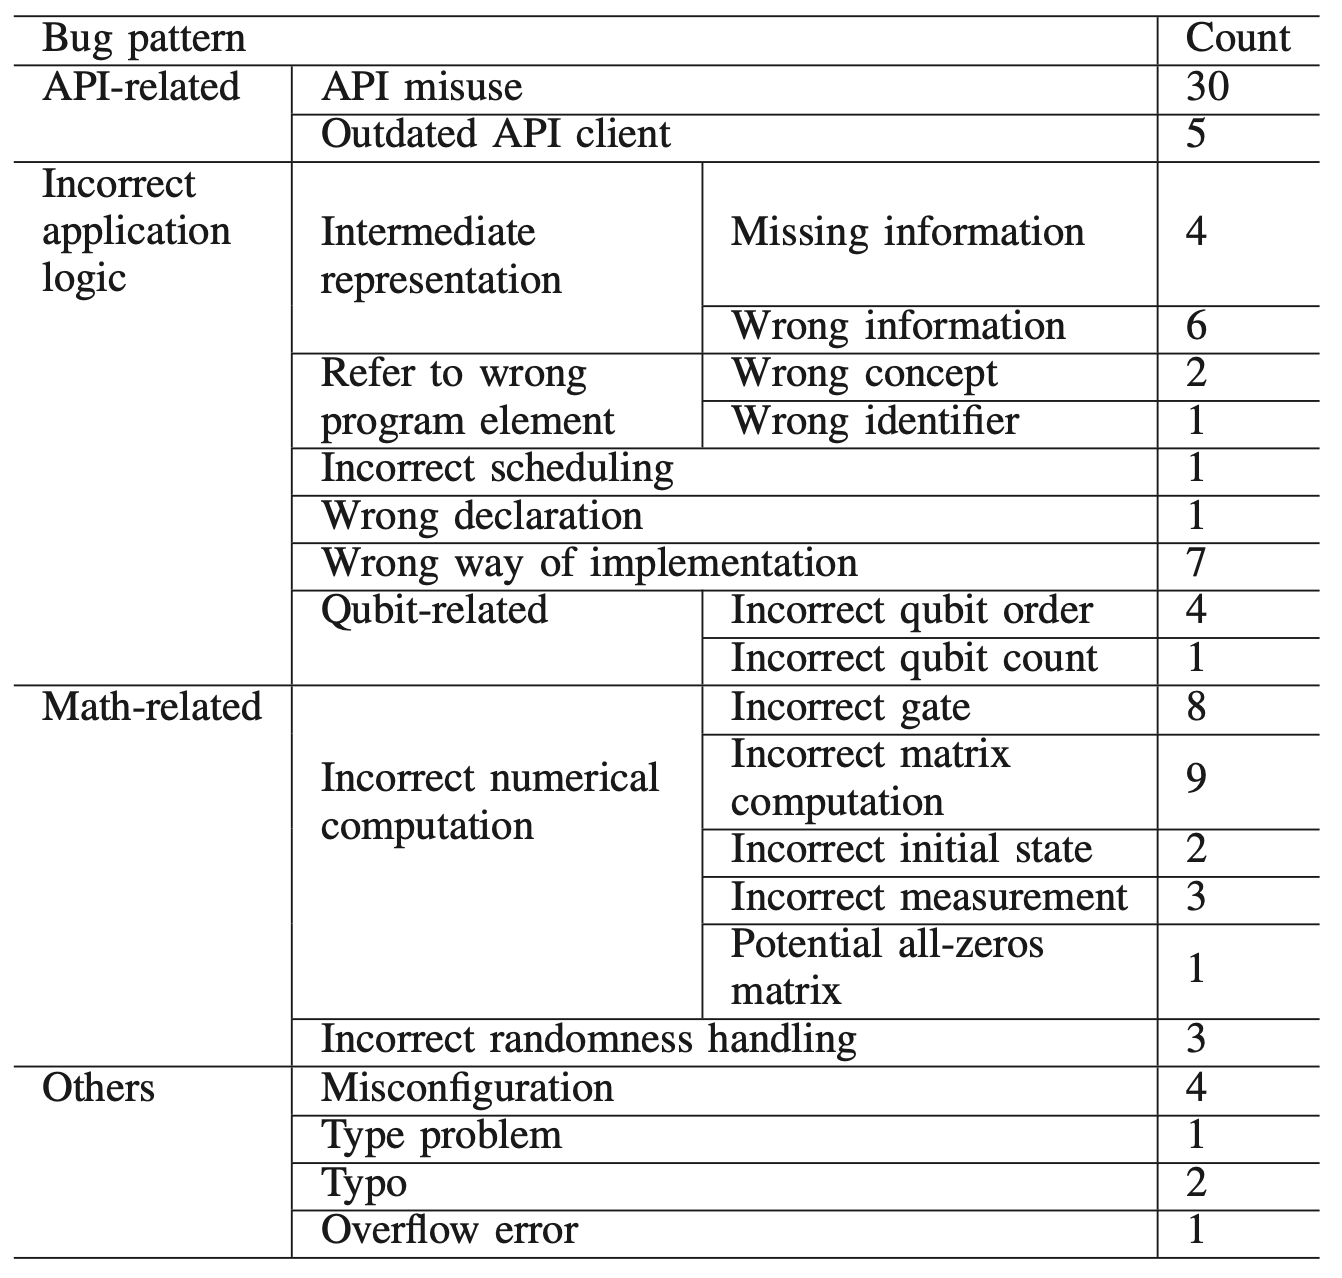
\includegraphics[width=0.46\textwidth]{TFM/photos/LuoBugPatterns.png}
        \caption{Bug patterns \cite{luo2022comprehensive}, following \cite{paltenghi2022bugs}} 
        \label{Fig:bugPatterns}
\end{figure}

\vspace{15pt}
\subsection{Debugging QC, 4 May 2022*}
Metwalli et al. presented the article with title: \textit{"A Tool For Debugging Quantum Circuits"} \cite{metwalli2022tool} where they introduced a debugging tool developed on Qiskit. The main drive was to provide users with a novel tool which help them debud their quantum programs.\newline

The authors present the general idea for this tool divided in three parts:
\begin{itemize}
    \item QP slicer: Which breaks a quantum program in different subprograms.
    \item Testing individual slices.
    \item Gate tracking.
\end{itemize}

The tool has been implemented as an extension of \textit{QuantumCircuit Class}, this way there was no need to create a new whole type. They included 2 new methods which adds \textit{breakBarrier()}, will help up slice the program vertically and \textit{gateInfo()} which provides tehe necessary information about a particular gate. It will introduce functions which will start the debug state, produce slices and obtain prositions and number of a particular gate in a circuit.\newline

Let us see what we include on each part of the tool and how it is going to work.
\begin{itemize}
    \item QP slicer: We are going to difference between two types, a vertical slicer which will divide the different slices on the QP and a horizontal slicer which will reduce the number of qubits of each subprogram, being able to slice the ones unused on each subprogram. The slicing could be accumulated, where each new slice it is added to the previous one.
    \item Testing each slice: The authors idea is to categorise each slide and there is a different testing technique for each category. The version presented categorises the slides by size of the circuit, type of gates involved and their possible effects over states entanglement. There is three different options for test cases: uniform superposition state, specific state or a symmetric state, GHZ, W and Dicke state supported.
    \item Gate tracking: When an error occurs, one of the possibilities is if the wrong gates have been implemented. Therefore, the authors included a gate tracking in the tool to help with the debugging of the problem.
\end{itemize}

The authors present an example on how would the slicer works and categorise the different slices, they take the triangle graph problem solver algorithm using Grover's algorithm. The evaluation has been done by the release of a beta version of the tool and it has been distributed within a group of quantum programmers with different levels of expertise in QC. The idea is to asses the capabilities of the tool for any level, including the installation and usage of the tool. The results received by surveys show that it makes it easier and less time consuming to locate the bug using the tool.\newline

The authors focus their next research on providing a larger tool which higher capabilities, including a more accurate categorisation criteria, expansion of gate tracking and develop an automated testing function for commonly used subroutines.

\vspace{15pt}
\subsection{QPs testing with MR; May 2022*}

Abreu et al. presented the article with title: \textit{"Metamorphic testing of oracle quantum programs"}\cite{abreu2022metamorphic} in May 2022. The idea of the authors is to tackle some of the main challenges and key difficulties in quantum computing testing. 
\begin{itemize}
    \item Unable to use methods with step-by-step monitoring.
    \item Quantum states in general are high-dimensional and difficult to interpret, limiting testing to debug misbehaving quantum programs.
    \item Non existent guidelines for quantum computing testing.
\end{itemize}

They propose metamorphic testing, MT, to mainly overcome the quantum measurement problem. MR will be specified in the quantum setting, avoiding to measure the quantum state. The proposed approach will show the process by applying it to a simple modular adder implementation, using Grover algorithm to speed up the testing process.\newline

The main idea is to obtain the MR that our implementation under test should fulfil and then find the way of expressing this on a simple quantum way. The authors in the paper they present $MR_0=x +_m 0 = x$, therefore they need to compare the equality of two integers. They will use different adder, as their proposal is under test, to obtain a result of that equality. They will obtain the complementary of one of them and perform the addition, therefore the result should be all bits to 1. \newline

Once the MR have been studied and proposed the approach, the authors study the difference between performing a classical or a quantum approach for verification of MR. Classical approach will raise two main concerns:
\begin{itemize}
    \item Do we need to implement the MR as quantum when we performing classical test to the MR?
    \item Is it possible to perform it in a quantum computing? Taking advantage then of quantum parallelism.
\end{itemize}

The authors then focus on the quantum approach for MR, with the main base on Grover's algorithm. They expressed how this can fit with Grover's algorithm as the metamorphic rule can be seen as a search function for the failing tests: $f(t)=1$ if the test $t$ fails the metamorphic rule indicated by $f$. Although, this approach faces two challenges:

\begin{itemize}
    \item Grover algorithm requires that the number of succeded tests are lower than half of the cases. If we are not in this maxim, Monte Carlo approach could be used or the search space could be increased by 1 qubit.
    \item Grover algorithm does not have to stop when a solution is found. Therefore the number of steps must be know beforehand and the authors propose an hybrid program to make sure we perform enough calls until results are obtained with high probability.
\end{itemize}

The authors apply directly this approach over the MR defined previously, obtain the expected results. Although, they would like to show how Grover's algorithm behaviour changes under the presence of bugs, therefore they introduce mutants. The results show how the algorithm finds a solution, and consequently we could affirm that it has found the mutant.

We can conclude now with the main contributions of this proposal and some of the challenges still beign faced as future work.

\begin{itemize}
    \item Metamorphic testing concepts can be applied in QP.
    \item The whole process is perform in the quantum realm.
    \item Validity of the approach under the experiments shown in the paper.
    \item Speed up versus classical approach on MR validation.
    \item Research needed on the extraction of adequate input test cases and application on different and more complex QP.
\end{itemize}

\vspace{15pt}
\subsection{MutTG; 08 July 2022*}

Wang et al. presented the article with title: \textit{"Mutation-Based Test Generation for Quantum Programs with Multi-Objective Search"}\cite{wang2022mutation} The authors adopted the same theoretical framework as they applied on \cite{ali2021assessing} and \cite{wang2021quito}, those papers were presented previously on ****. Defining two new concepts of possible output failures directly connected to the names of the appropriate oracles.\newline

The authors propose a search-based approach, called MutTG, that tries to generate the minimal test suite killing as many mutants as possible, aiming for all non-equivalent mutants. They define an individual of the search as a set of $k$ elements, if there is $k$ mutants. Where this elements provide from the testing domain or anything else not in the testing domain. This will represent possible set of tests with cardinal lower than $k$.\newline

MutTG applies and algorithm on each set of test cases. Saving dictionaries if a test killed the mutant or if it didn't, once one mutant is killed, the algorithm loop with the following mutant without testing the remaining test cases. We will call $KM$ the dictionary of pairs $<t,{M_{1},..,M_{n_{t}^{kill}}}>$, if $t$ killed $m_{i}$. And, analogous $NKM$, if $t$ does not kill $m_{j}$. This dictionaries are global and they will be used in the following executions, starting from empty dictionaries.\newline

The authors idea is to asses with this dictionaries if a mutant is highly likely to be an equivalent mutant, they create this functions:
\begin{itemize}
    \item $discFactor$(Mutant, $NKM$): The discount factor is going to be the percentage between the number of tests that have not killed the mutant and the number of possible test in the domain.
    \item $notKilledScore$(Mutant,search, $KM$, $NKM$): The function gives a score to each mutant:
        \begin{itemize}
            \item[$\cdot$] 0, if it has been killed on this search.
            \item[$\cdot$] 1, if it hasn't been kill on this search but it has been killed previously.
            \item[$\cdot$] 1 - $discFactor$, otherwise.
        \end{itemize}
    \item $f_{not\_killed}$(search): Sum of all $notKilledScore$.
\end{itemize}

Experiment design:

\begin{itemize}
    \item Five quantum programs: BV, QRAM, invQFT, AddSquare, ConditionalExecution.
    \item Three set of mutants by difficulty: 
        \begin{itemize}
            \item[$\cdot$] Easy, killed by at least $25\%$ inputs of input domain.
            \item[$\cdot$] Medium, killed by at least $1.26\%$ and less than $25\%$ inputs of input domain.
            \item[$\cdot$] Hard, killed by at most $1.26\%$ inputs of input domain.
        \end{itemize}
    \item Statistical test used for $wodf$ oracle: Pearson Chi-square test with $\alpha= 0.01$ as the significance level.
    \item Three search approach: MutTG, MutTG without $discFactor$ and Random Search, in particular NSGA-II.
    \item Three metrics:
        \begin{itemize}
            \item[$\cdot$] $Hypervolume$: quality indicator, obtain from \cite{shang2020survey}. The higher, the better.
            \item[$\cdot$] $MNNKM$: minimum number of not killed non-equivalent mutants. The lower, the better.
            \item[$\cdot$] $TSS_{MNNKM}$: minimum size of the test suite achieving $MNNKM$. The lower, the better.
        \end{itemize}
    \item Statistical test within metrics: Mann–Whitney U test with significance level $0.05$ and Vargha and Delaney’s $\hat{A}_{12}$ statistics as effect size measure.
\end{itemize}

Research questions and results:

\begin{itemize}
    \item[] \textbf{RQ1} What is the influence of the discount factor on the effectiveness of the search of MutTG?
        \begin{itemize}
            \item MutTG shows as the most effective if there is any difference between them.
            \item The effectiveness improvement can be reflected on the experiments with higher difficulty which has a higher amount of equivalent mutants.
        \end{itemize}
    \item[] \textbf{RQ2} How does the difficulty of the benchmarks affect the effectiveness of MutTG?
        \begin{itemize}
            \item The authors results shows that difficulty has a big impact on test suite size, even when sometimes the value could be really low, there is cases where not even all non-equivalent mutants are killed even with more than 500 generations. 
        \end{itemize}
    \item[] \textbf{RQ3} How does the number of equivalent mutants in the targeted mutants set affect the effectiveness of MutTG?
        \begin{itemize}
            \item It is more challenging to kill non-equivalent mutants if the number of equivalent ones are lower, as expected just due to the number of mutants in place.
        \end{itemize}
\end{itemize}

\vspace{15pt}
\subsection{QMutPy; 29 July 2022}
\label{Ch3.2.4:QMutPy}

Check add ons on 15-19 November 2021 \cite{fortunato2022qmutpy}

The initial approach we are presenting was authored by Fortunato, D. et all in 2022 in their article titled "\textit{Mutation testing of quantum programs: A case study with qiskit}"\cite{fortunato2022mutation}. In this work, they explore mutation testing on QP with the extension of the MutPy library by introducing new quantum mutation operators. This article can be divided into two distinct sections. The first section focuses on the introduction of QMutPy and the initial experiments. The second section delves deeper into the previous results to identify potential causes and solutions. The authors implement some of these solutions to determine if they are on the right path. \newline

First, let us understand what QP are going to be tested and why did the authors choose this library. The oracle problem was one of the challenges discussed earlier, where given an input, we need the expected behaviour. In this article, the authors have decided to prioritise and initially focus on this new approach for QP testing. To accomplish this, they opted to use Qiskit-Aqua's repository, which has since been moved to Qiskit-Terra \footnote{\url{https://github.com/Qiskit/qiskit-aqua/\#migration-guide}}.This repository provides the implementation of 24 QP along with their respective test suites. In these repository, you can discover a variety of programs, including pure classical, hybrid, and pure quantum programs.\newline

Similarly, they carefully selected the tool they believed would be the most suitable for implementing their ideas about quantum mutation testing. Their criteria included support for Python programs, testing frameworks, mutation operators, and the capability to generate appropriate reports. For that reason, they choose MutPy, as it fulfils their specific needs. Now, let us see how they develop these new quantum mutation operators, expanding the library mentioned earlier and naming it QMutPy.\newline

They have introduced in QMutPy 5 quantum mutation operators, QMO:
\begin{itemize}
    \item Quantum gate replacement, QRG.
    \item Quantum gate deletion, QRD.
    \item Quantum gate insertion, QRI.
    \item Quantum measurement insertion, QMI.
    \item Quantum measurement deletion, QMD.
\end{itemize}

\vspace{5pt}
These new operators are designed to capture the main errors that can occur during the implementation of an algorithm. The key concept around QMO is gate equivalence. We will consider two gates to be syntactically equivalent if and only if the number and type of the arguments are identical. The authors have identified 40 gates with at least one syntactical equivalent gate. As an example, gate h would have the following equivalent gates: x, y, z, i, id, s, sdg, sx, t and tdg. In their article \cite{fortunato2022mutation}, the authors illustrated all equivalence gates in Figure 1.  \newline

There is no need to provide an explanation for the mutant operators, as they are inherently self-explanatory.  However, let us dig into a more comprehensive understanding of gate operators. As mentioned earlier, the fundamental concept that makes these operators effective is gate equivalence. Whenever we encounter a gate addition (denoted by ".append()"), and we intend to employ QRG or QRI, we will either replace the existing gate with a syntactically equivalent one or simply add a new gate that preserves the syntax of our program. The process will generate as many mutants as there are syntactically equivalent gates. All of these modifications are implemented using Python's Abstract Syntax Tree (AST).\newline

QMutPy workflow, analogous to MutPy:
\begin{itemize}
    \item Loads QP source code and test suite.
    \item Executes test suite on the unmutated QP.
    \item Applies mutant operators, including QMO.
    \item Executes test suite on all mutated QP and provides a summary of results.
\end{itemize}

Because the works in quantum mutation \cite{wang2021qdiff}\cite{mendiluze2021muskit}\cite{ali2021assessing} were in a preliminary state, the authors opted to compare MutPy and QMutPy by running experiments on the same set of quantum programs and test suites. The experiment's metrics will be assessed through two distinct approximations of the mutation score. The first one follows the classical interpretation\cite{jia2010analysis}, while the second allows for the potential achievement of 100\% mutantion score. This will be achieved by excluding from the total mutants generated those that haven't been executed.\newline

The authors will perform when needed Kruskal-Wallist non-parametric test with $p=0.01$ and Cohen's $d$ effect-size measure on the results reported by QMutPy to evaluate the statistical significance.\newline

Let us conclude by highlighting the key contributions and outcomes of these experiments:

\begin{itemize}
    \item Expansion of the set of mutation operators for quantum programs, implemented in QMutPy.
    \item Introduction of gate equivalence definition based on the number and type of arguments.
    \item QMutPy generates quantum mutants for 11 out of 24 QPs. The remaining 13 QPs should exclude quantum gates and measurements. On average, 4 lines of code (LOCs) are mutated, resulting in 13 mutants and 64 mutants per QP. MutPy, on the other hand, generates mutants for all programs with an average of 64 LOCs mutated, 3 mutants, and 147 mutants per QP.
    \item QMutPy's performance in mutant creation is not statistically significantly lower than MutPy when considering the potential number of classical vs quantum mutations per QP.
    \item Test suits may only focus in the quantum part of the program, as evidenced by the difference in mutation scores between classical and quantum mutations and the type of killing (error vs test assertion).
    \item QMutPy exhibits reduced efficiency in creating quantum mutants. One proposed solution involves defining new operations in Python AST for quantum gates to enhance creation time.
\end{itemize}

As mentioned earlier, the authors delved into potential enhancements for these results, particularly focusing on test suites. They concentrated on two criteria for improvement: coverage and test assertions. By selecting specific programs for each test, they identified why mutants survived and implemented new assertions or tests as necessary. Therefore, the augmentation of test suites and assertions resulted in an increased mutation score for the studied programs.

\begin{itemize}
    \item The mutation score for $hhl$’s rose from $50\%$ to $100\%$ (with coverage increasing from $86.55\%$ to $89.16\%$), and for $vqc$’s, it increased from $0\%$ to $50\%$ (coverage rising from $93.26\%$ to $94.43\%$).
    \item In the case of Shor's algorithm, the original test suite achieved a $53.34\%$ mutation score, whereas the augmented test suite reached $72.81\%$.
\end{itemize}

\vspace{15pt}
\subsection{QuMu; 13 October 2022*}

García de la Barrera et al. present \textit{"Quantum Software Testing: Current Trends and Emerging Proposals"} \cite{de2022quantum} in 2022 as one of the chapters in the book \textit{Quantum Software Engineering} \cite{serrano2022quantum}. This chapter introduces a quick overview of the State of Art of testing in Quantum Computing. We will focus in the \textit{Quantum Mutation Support Tool, QuMu} prototype presented by the authors within this chapter.\newline

They use Quirk\footnote{\url{https://algassert.com/quirk}}, which is a quantum circuit simulator. Each circuit is represented by an ordered set of columns and on each column an ordered set of gates. This structure will be used to save the position which allow a mutation. They defined an abstract operation, \textit{isApplicableTo}, for this matter. Which allows identifies which gates can be passed as parameters, and therefore creates a mapping of gates which could be mutated.\newline

The authors define several mutation operators, grouped in different categories, fully develop in Table 9.1 in \cite{de2022quantum}:

\begin{itemize}
    \item Initialisation: Change initial value, first gate duplication and further gate duplication.
    \item Wrong gate.
    \item Missing gate: One-qubit gate removal, multi-qubit gate removal and control gate removal.
    \item Bridging faults: Swap controls and controlled qubits.
    \item Entanglement faults: Wrong entanglement initialisation, entanglement corruption, force unentanglement and force entanglement.
\end{itemize}

The process is split between two engines:
\begin{itemize}
    \item Mutant generation: Iterates over selected mutation operators using the map explained previously.
    \item Mutant execution: Uploads the mutated circuit onto the Quirk website, executes a simulation, downloads and saves the results in the database.
\end{itemize}

They use distribution matrixes to compare results to identify killed, alive and injured mutants. This last ones identifies as the one who produce the same distribution matrix but leave the qubits with a different phase, we can observe this in Figure \ref{Fig:QuMUInjured}. This prototype includes a mutants results analyser.

\begin{figure}[H]
        \centering
        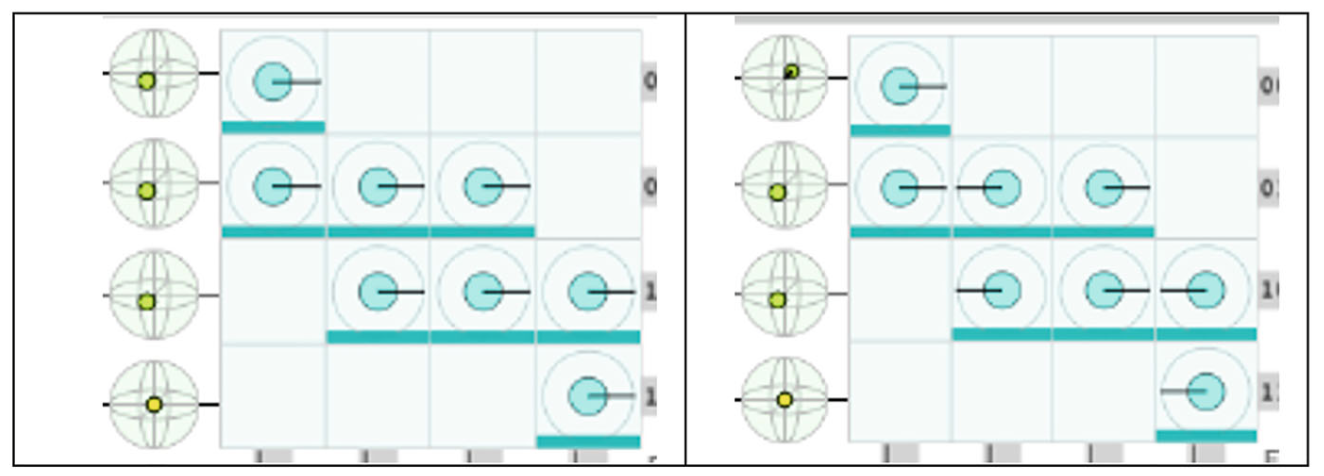
\includegraphics[width=0.9\textwidth]{TFM/photos/QuMuInjured.png}
        \caption{Injured mutant \cite{de2022quantum}} 
        \label{Fig:QuMUInjured}
\end{figure}

\vspace{15pt}
\subsection{Shor's correctness with MR; 09 November 2022*}

Nuno Costa et al. presented in 2022 the paper with title: \textit{"Asserting the correctness of Shor implementations using metamorphic testing"} \cite{costa2022asserting}. Where they used metamorphic testing to try and prove the correctness of the well known Shor's algorithm.\newline

Firstly the authors delve into Shor's algorithm, this is needed due to metamorphic testing  characteristics, where to defined adequate metamorphic rules, MR, is important to understand the algorithm we facing. Let us see their proposal for MR:
\begin{itemize}
    \item In the domain of \textit{number factoring} where $p$ is a given prime number, $q_{1}$ is a given number, and $f(x)$ represents the set of factors of $x$, the following MR, named Add Prime, should hold: if $q_{2}$ is equal to $q_{1}\times p$ then $f(q_{2}) \backslash f (q_{1}) \subseteq {p}$.
    \item In the domain of number factoring where $q_{1}$ and $q_{2}$ are given numbers and $f(x)$ represents the set of factors of $x$, the following MR, named Multiply Factors, should hold: if $q_{3}$ is equal to $q_{1}\times q_{2}$ then $f(q_{3})=f(q_{1})\cup f(q_{2})$.
\end{itemize}

The authors then proceed to implement MR \textit{Add Prime}, and do some experimental studies using mutants. They remark that with the current number of qubits in real quantum systems, they are not able to reproduce the experiments there for Shor's algorithm due to the high qubit required. Due to Shor's nature as non-deterministic algorithm, the results could still fail the test, even with a correct implementation. For this reason the authors include a threshold of 20 iterations, taking as pass if one of them fulfils the MR. they conclude that due to this challenges further research is needed in this approach, although with the appropriate threshold, they can observe how the MR detect implementation failures. 

\vspace{15pt}
\subsection{Automatic test circuit generation; 09 November 2022*}

Garcia et al. presented a preliminary work at the end of 2022 tittle: \textit{"Automatic generation of test circuits for the verification of Quantum deterministic algorithms"} \cite{garcia2022automatic}. The authors want to introduce test cases to be run within the machine. The idea is to embed the quantum circuit under test, CuT, in a QP that checks if the expected output is the same than the computed output, producing a verdict for the test case and not the outputs.\newline

They reproduce this idea with the adder algorithm for two qubits, using a correct test suite and a modified one to observe how the program shows the non matching results, generating a quantum test circuit, QTC.\newline

In my opinion, one of the points to highlight from this approach is the increased number of qubits used, as we can see on Figure \ref{Fig:GarciaAdder}. The original adder needed 4 qubits and the whole system to verify the test suite needs 9. A similar approach was used previously by Abreu et al. in \cite{abreu2022metamorphic} to represent the output of a metamorphic rule.

\begin{figure}[H]
        \centering
        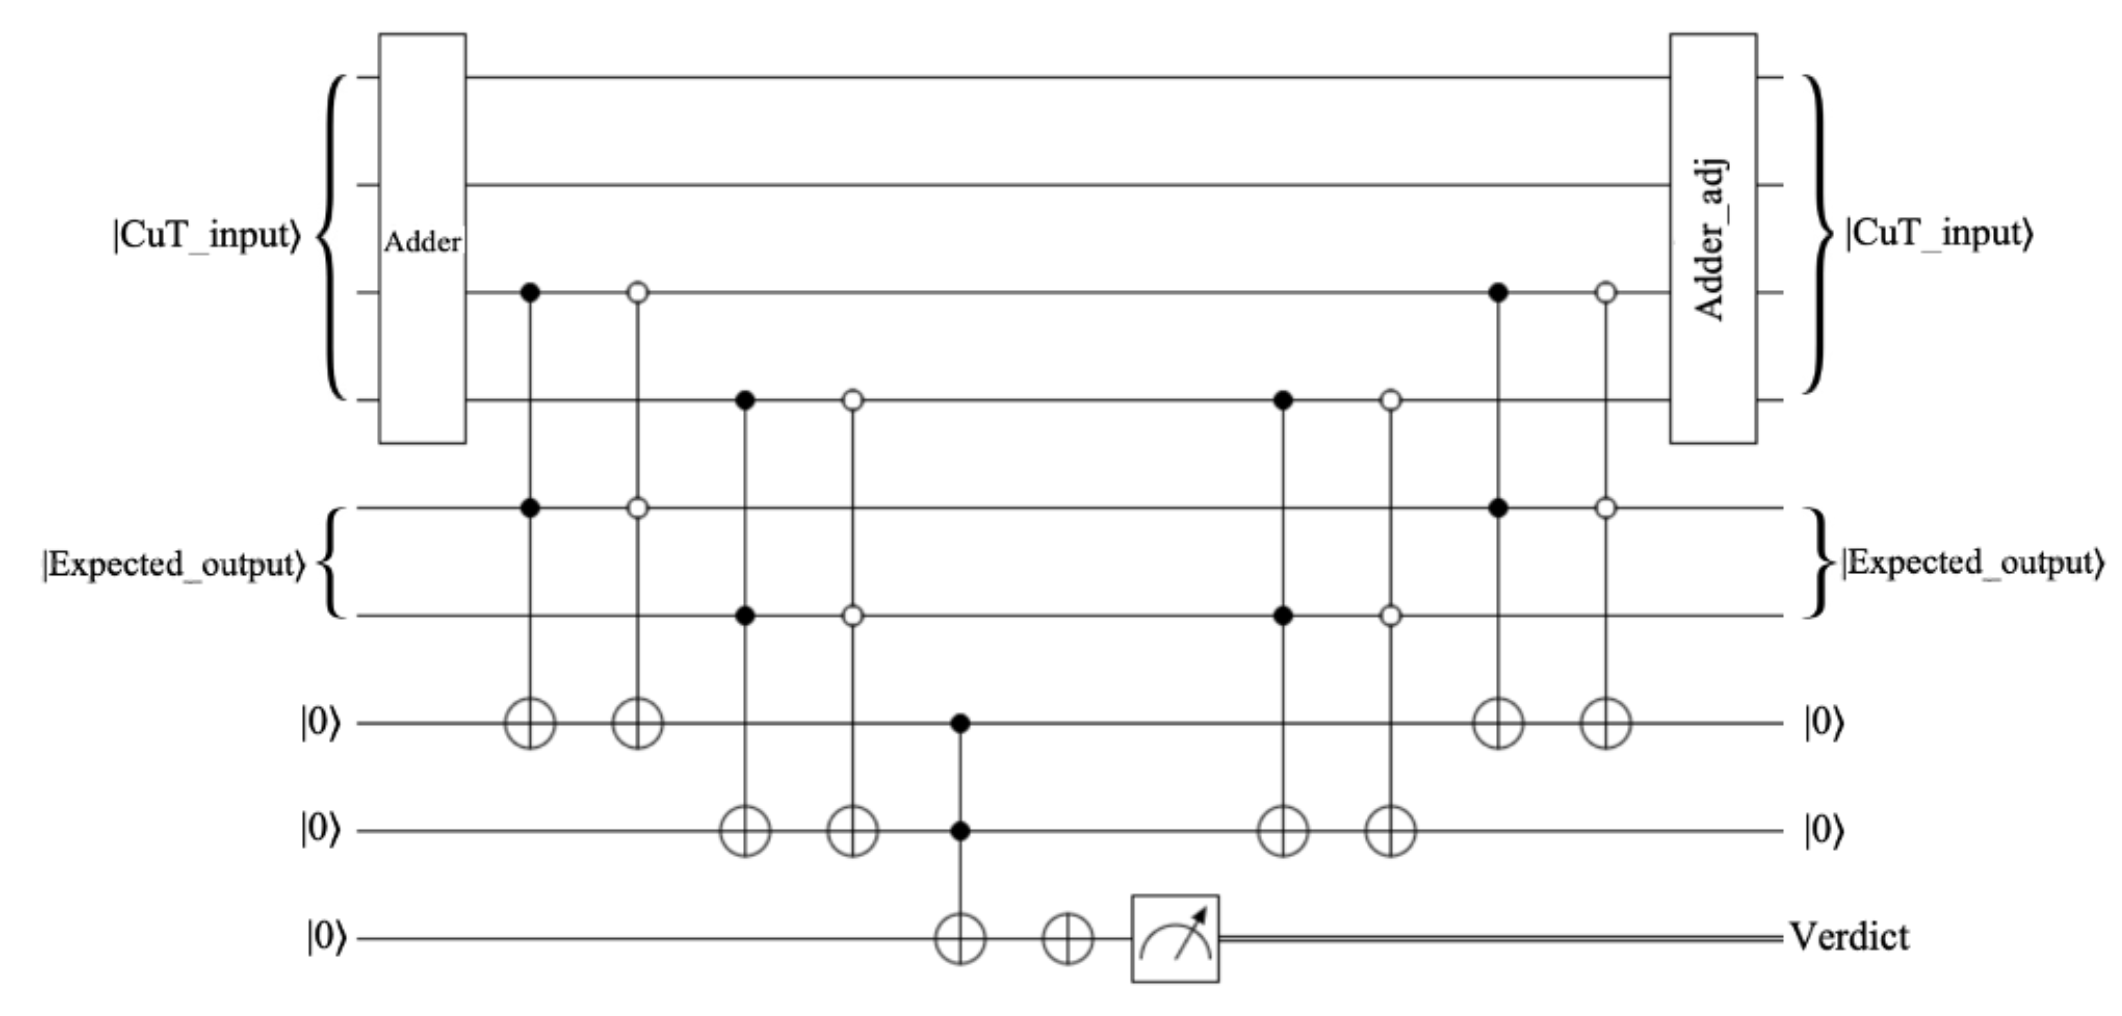
\includegraphics[width=0.9\textwidth]{TFM/photos/GarciaAdder.png}
        \caption{Adder QTC \cite{garcia2022automatic}} 
        \label{Fig:GarciaAdder}
\end{figure}

There is a new version of this paper where the authors delve into this approach and have new study cases, the title is: \textit{"Automatic generation of test circuits for deterministic quantum algorithms"} \cite{garcia4421955automatic} which is still on pre print state.

\vspace{15pt}
\subsection{Coverage Criteria for Quantum Software Testing; 01 March 2023*}

Ajay Kumar presented the paper titled: \textit{"Formalisation of Structural Test Cases Coverage Criteria for Quantum Software Testing"} \cite{kumar2023formalization} where he wanted to introduce the concept of cyclomatic complexity in quantum to give an understanding of the quantum testing complexity, the original concept was introduced by McCabe in 1976\cite{mccabe1976complexity}. The author define as \textbf{cyclomatic complexity} for quantum, the number of independent paths and paths generated due to the superposition of each control qubit. We will see how this concept will lead us to a structural coverage criteria to test QPs.\newline

McCabe\cite{mccabe1976complexity} introduced the concept of cyclomatic complexity based on graph theory. Cyclomatic complexity is a quantitative metric for finding the number of independent paths in a control flow graph. If we have a control flow graph with n nodes, e edges, and p-connected components then $e-n+2p$ is its complexity. He proved that the cyclomatic complexity of n-different modules of a program is equal to the sum of the cyclomatic complexity of all modules.\newline

If we focus now into quantum, we have 3 different possibilities for control qubits:

\begin{itemize}
    \item Control qubit is $|1\rangle$ or $|0\rangle$, the we are in the same situation as classical computing, with its complexity being defined by $e-n+2p$.
    \item Control qubit is in superposition. Then we need to consider a test case that cover that state. If there is $c$ instances of control qubits in the QP, then cyclomatic complexity will be $e-n+2p+c$
\end{itemize}

Let us see now different control flow graphs for different gates, Figure \ref{FIG:KumarCFG}.

\begin{figure}[H]
    \centering
    \begin{subfigure}[H]{0.48\textwidth}
        \centering
        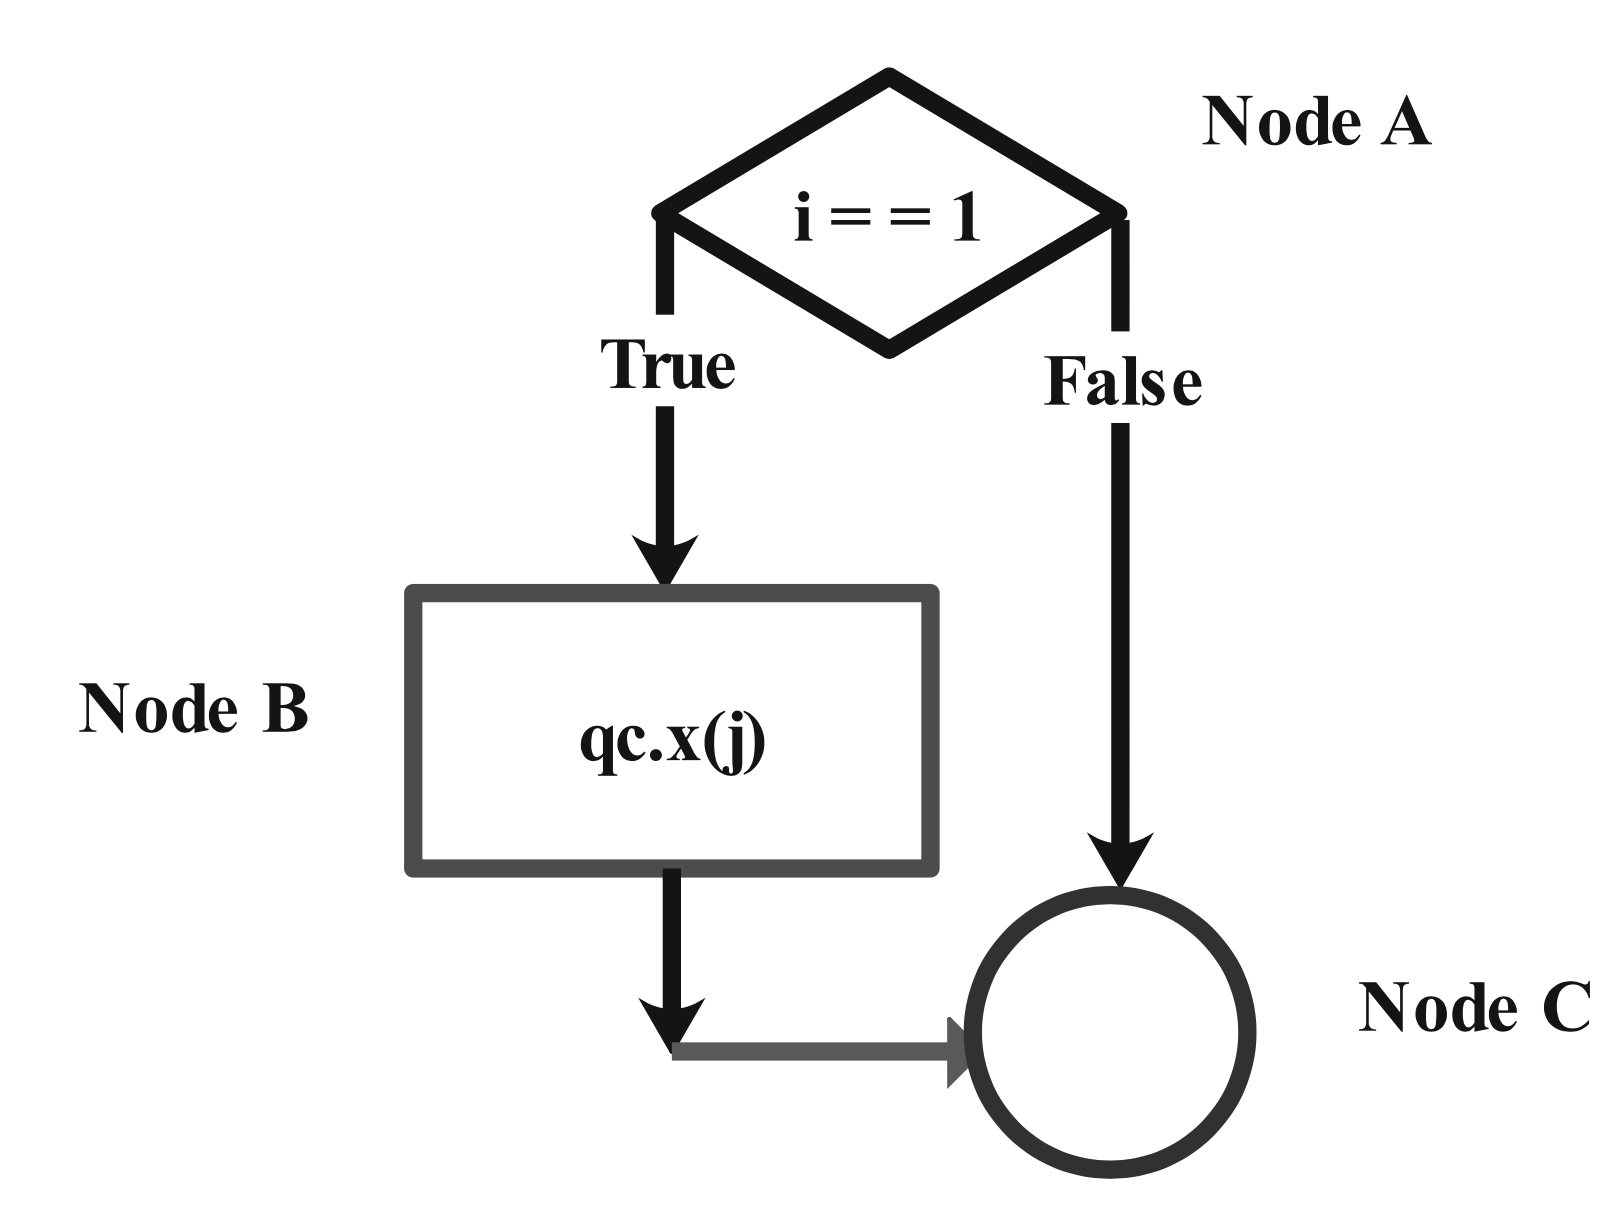
\includegraphics[width=\textwidth]{TFM/photos/KumarCNOT.png}
        \caption{CNOT $(i,j)$ control flow graph.} 
        \label{Fig:KumarCNOT}
    \end{subfigure}
    \hfill
    \begin{subfigure}[H]{0.48\textwidth}
        \centering
        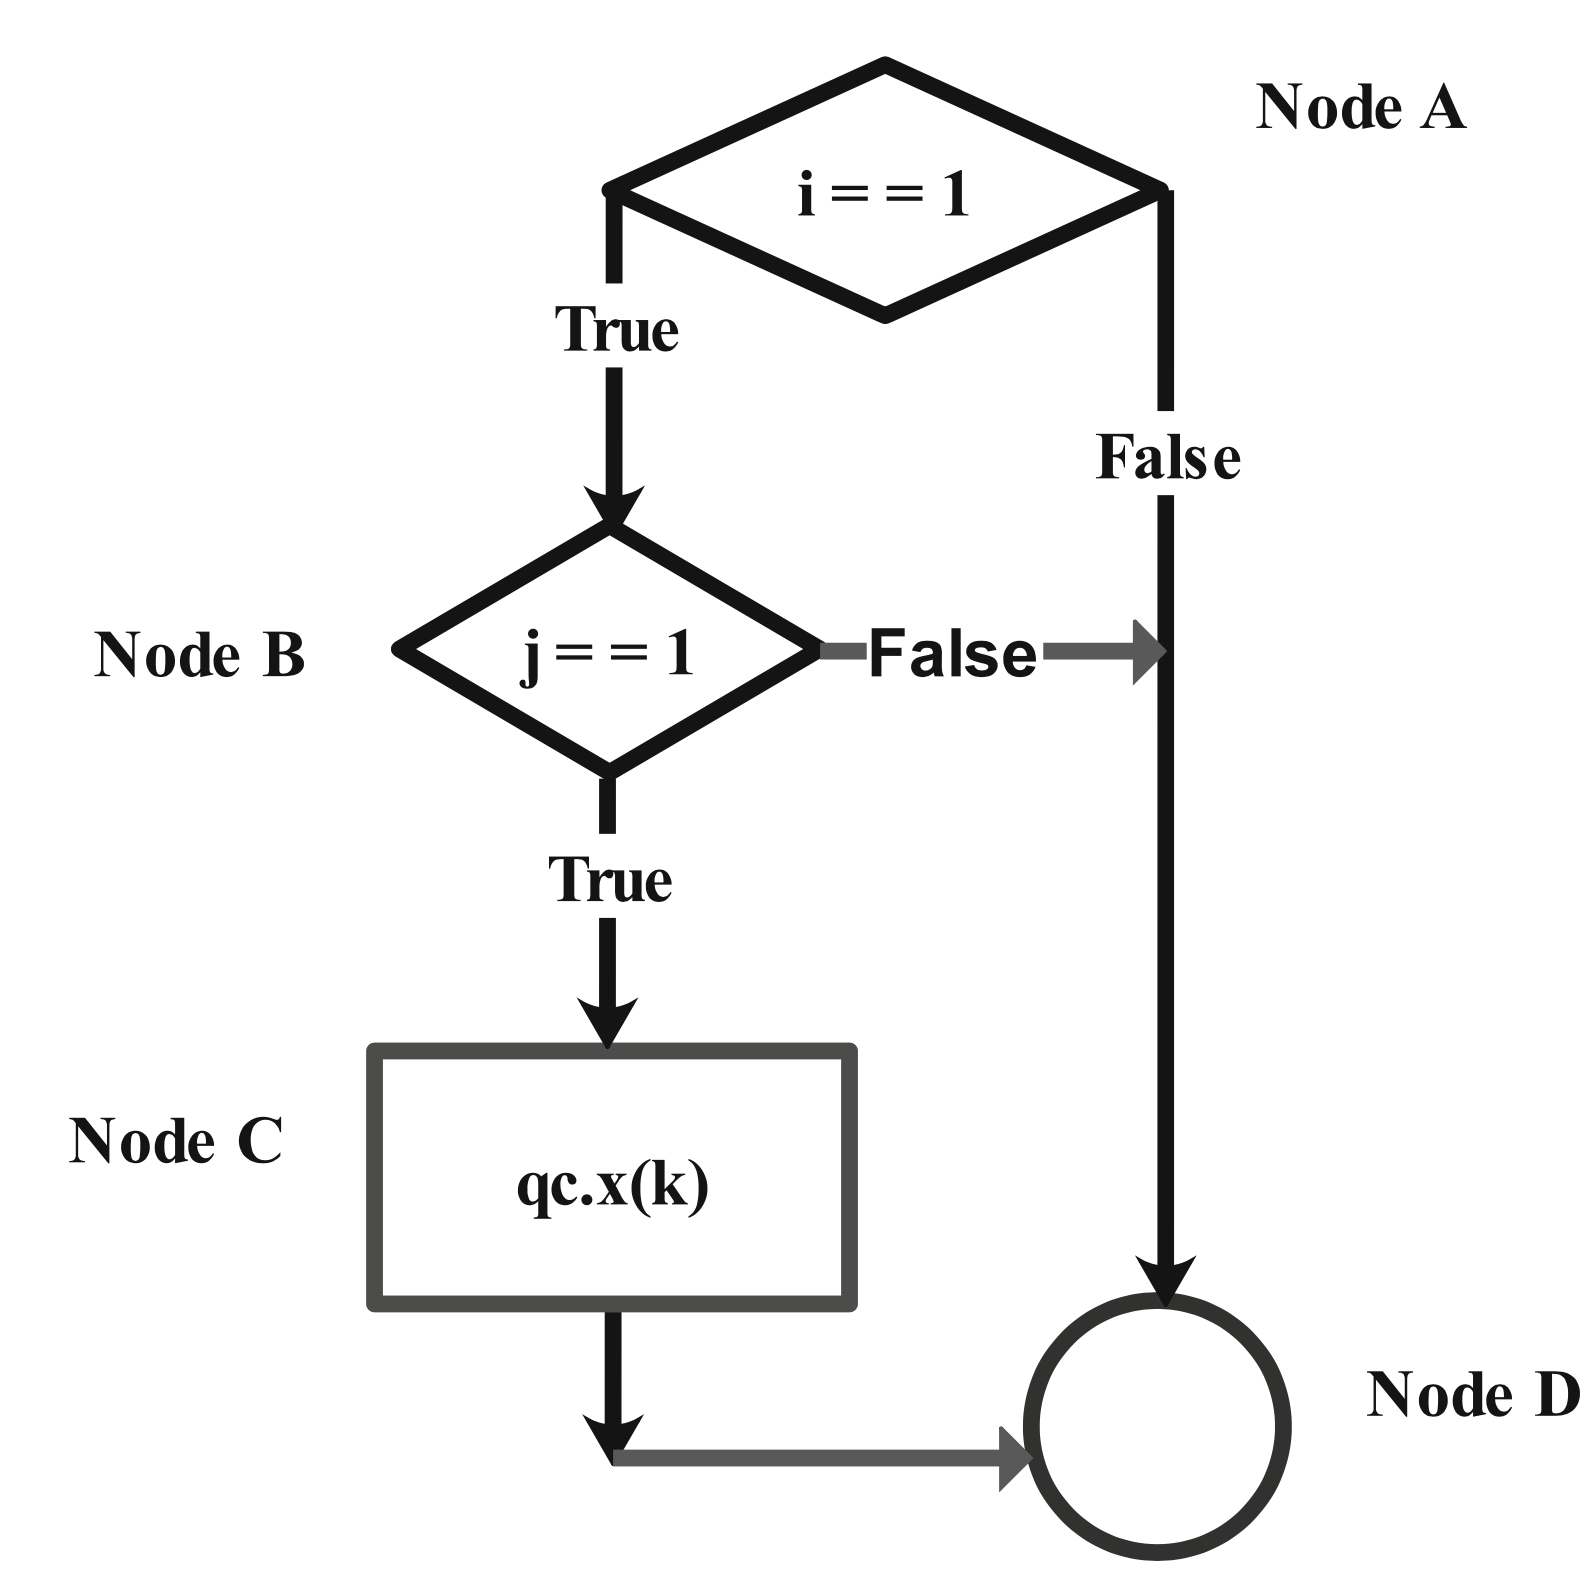
\includegraphics[width=\textwidth]{TFM/photos/KumarToffoli.png}
        \caption{Toffoli $(i,j,k)$ control flow graph.} 
        \label{Fig:KumarToffoli}
    \end{subfigure}
        \caption{Two possible control flow graphs \cite{kumar2023formalization}. }
    \label{FIG:KumarCFG}
 \end{figure}

Let us see the possible paths in Figure \ref{Fig:KumarToffoli} :
\begin{itemize}
    \item Linear Independent Path 1: A, B, C, D.
    \item Linear Independent Path 2: A, D.
    \item Linear Independent Path 3: A, B, D.
    \item Superposition Path 1 (Control qubit $|i\rangle$ in superposition): A, $\alpha|\text{B}\rangle\text{CD}+\beta|\text{B}\rangle$ where $\alpha,\beta \in \mathbb{C}$ and $|\alpha|^{2}+|\beta|^{2}=1$.
    \item Superposition Path 2 (Control qubit $|j\rangle$ in superposition): A, B, $\alpha|\text{C}\rangle\text{D}+\beta|\text{C}\rangle$ where $\alpha,\beta \in \mathbb{C}$ and $|\alpha|^{2}+|\beta|^{2}=1$
\end{itemize}

The authors then present some coverage criteria for 1, 2 or more qubits, taking into accounts what gates are in use and with 2 assumptions: all gates are reachable and QP optimised, i.e. not two consecutive H gates. Concluding that this criteria should be explored as they have just been introduced towards cyclomatic complexity and the criteria only covers quantum control.

\vspace{15pt}
\subsection{Testing Multi-Subroutine Quantum Programs; 4 Jul 2023*}

Peixun Long and Jianjun Zhao unveiled their paper, titled \textit{"Testing Multi-Subroutine Quantum Programs: From Unit Testing to Integration Testing"} \cite{long2023testing}, in July 2023, building upon their earlier work presented in \cite{long2022testing}. Their objective is to introduce novel testing techniques tailored to the unique challenges and characteristics associated with multi-subroutine quantum programs.\newline

Until now, the majority of research efforts have predominantly concentrated on testing small or fixed-scale quantum programs, without the complexities inherent in practical quantum programs featuring multiple subroutines and a blend of classical-quantum inputs and outputs. The authors aim to bridge this gap in the existing literature, delving deeper into the intricacies posed by such multifaceted quantum programs.\newline

The authors focused their research in the following RQ:
\begin{itemize}
    \item[] \textbf{RQ1}: What are the critical properties of multi-subroutine quantum programs, and how do they impact testing?
    \item[] \textbf{RQ2}: Are our unit testing design strategies effective for testing various quantum subroutines?
    \item[] \textbf{RQ3}: Is it necessary to cover both classical and superposition states as inputs to ensure adequate test coverage?
    \item[] \textbf{RQ4}: How effectively does the Superposition-Cover-All-Qubit (SCAQ) criterion reveal bugs in quantum programs?
    \item[] \textbf{RQ5}: Are our testing design strategies effective for testing multi-subroutine quantum programs?
\end{itemize}

To answer these questions, they propose Q-UML diagrams to define unit testing and integration testing between the subroutines.
\begin{itemize}
    \item[] \textbf{A-RQ1}: Focused on the approach to a QP from different perspectives: Program structure, subroutines, IO types. The authors defined four IO types in subroutines: Classical, Generate-Quantum, Detect-Quantum and Transform, represented in the Figure \ref{Fig:IOTypes}.
    \item[] \textbf{A-RQ2}: From IO types showed in RQ1, the authors propose 17 subroutines to cover all four types. They design a unit testing plan for each subroutine, this plans could be seen in Table 5, Section 8 of \cite{long2023testing}.
    \item[] \textbf{A-RQ3/4}: They proceed with experiments in the subroutines \textit{CRk, Teleport, Empty, Reverse, MultiSWAP} and \textit{QFT} using mutation testing. They acquire as mutation operators: quantum gate (GM), subroutine(SM), classical(CM) and measurement mutation(MM). Being CM and SM two new mutations types no used in previous research. To be able to answer the specific questions, they group the input in three types: classical input (CI), random two-value superposition input (RTI) and complementary superposition input (CSI).\newline
    From the experiments we can observe that the trigger rate is higher for RTI than CI and therefore the necessity of covering classical and quantum inputs. CSI has the highest trigger rate giving this an answer to RQ4 where a larger extent of superposition input states produces better results.
    \item[] \textbf{A-RQ5}: The idea is to prove this approach for QPs. To evaluate RQ5, the authors propose three case studies: Quantum phase estimations, Shor's algorithm and Linear system solver. The aim of choosing this QPs is the variety of subroutines included on each. The authors present for each case their corresponding Q-UML diagram to help them delve into the testing design. They obtained the following insights:
    \begin{itemize}
        \item[$\cdot$] In the top-down integration, quantum subroutines with an IO type of "classical" can be substituted with equivalent classical subroutines.
        \item[$\cdot$] If feasible, it is recommended to prioritise the adoption of transform-based methods for checking the running output.
        \item[$\cdot$] A recommended testing approach is systematically increasing the testing scale, starting from small-scale scenarios and gradually progressing to larger ones.
    \end{itemize}
\end{itemize}

\begin{figure}[H]
        \centering
        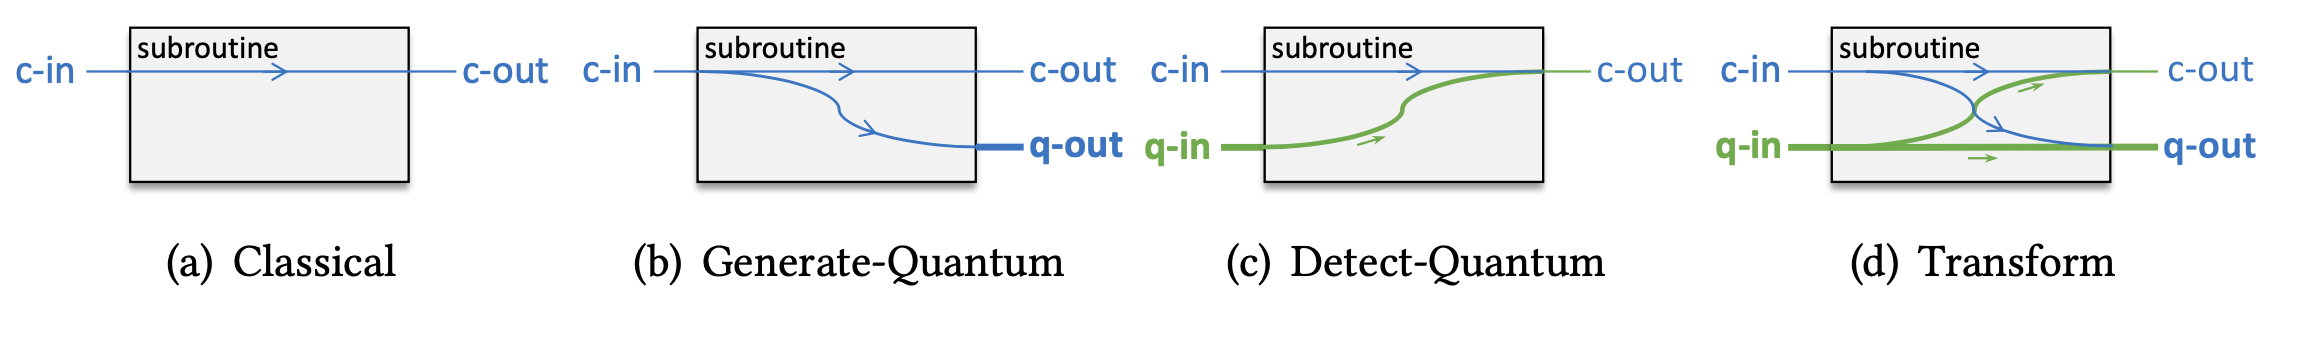
\includegraphics[width=0.7\textwidth]{TFM/photos/LongEqIOTypes.png}
        \caption{IO types \cite{long2023equivalence}} 
        \label{Fig:IOTypes}
\end{figure}

\vspace{15pt}
\subsection{Black-Box testing of QP; PrePrint}

Equivalence, Identity, and Unitarity Checking in Black-Box Testing of Quantum Programs \cite{long2023equivalence}

\vspace{15pt}
\subsection{Tool for equivalent mutants; PrePrint}

Development of a tool for finding equivalent mutants in quantum program: a perspective to measure the quality of quantum software. \cite{kumar2022development}

\section{Future work}
\label{Ch3.3:FutureWork}
